\documentclass[twoside,openright,titlepage,fleqn,pointlessnumbers,headinclude,%1headlines,%
12pt,a4paper,BCOR5mm,footinclude,cleardoubleempty,abstractoff]{scrreprt}


\listfiles

\newcommand{\myTitle}{Konzeption und Realisierung einer transparenten
Multiprotokoll Service Engine\xspace}
\newcommand{\myDegree}{Bachelor Informatik\xspace}
\newcommand{\myName}{David L\"ucke\xspace}
\newcommand{\myProf}{Prof. Dr. C. Pleier\xspace}
\newcommand{\myFaculty}{Fakult\"at f\"ur Informatik und Mathematik\xspace}
\newcommand{\myDepartment}{Put data here\xspace}
\newcommand{\myUni}{\protect{Hochschule M\"unchen\\Munich university of
applied sciences}\xspace}
\newcommand{\myLocation}{M\"unchen\xspace}
\newcommand{\myTime}{11. M\"arz 2010\xspace}
% \newcommand{\myVersion}{Version \xspace}

\usepackage[utf8]{inputenc} 
\usepackage[ngerman,american]{babel}           
\usepackage[square,numbers]{natbib} 
\usepackage[fleqn]{amsmath} % math environments and more by the AMS 

\usepackage{classicthesis-ldpkg}
\usepackage{url}
\usepackage{pdfpages}

\usepackage[eulerchapternumbers,listings,%pdfspacing,%
            subfig,beramono,eulermath,parts]{classicthesis}

\newlength{\abcd} % for ab..z string length calculation
\newcommand{\myfloatalign}{\centering} % how all the floats will be aligned
\setlength{\extrarowheight}{3pt} % increase table row height

\captionsetup{format=hang,font=small}

\lstset{language=[LaTeX]Tex,%C++,
    keywordstyle=\color{RoyalBlue},%\bfseries,
    basicstyle=\small\ttfamily,
    %identifierstyle=\color{NavyBlue},
    commentstyle=\color{Green}\ttfamily,
    stringstyle=\rmfamily,
    numbers=none,%left,%
    numberstyle=\scriptsize,%\tiny
    stepnumber=5,
    numbersep=8pt,
    showstringspaces=false,
    breaklines=true,
    frameround=ftff,
    frame=single,
    captionpos = b
    %frame=L
}

% \lstdefinelanguage{spring}
% 	{morekeywords={name, value, ref},
% 	3,
% 	sensitive=false,
% 	morecomment=[s]{<!--}{-->},
% 	morestring="`[b]"',
% }

\hypersetup{%
    colorlinks=true, linktocpage=true, pdfstartpage=3, pdfstartview=FitV,%
    % uncomment the following line if you want to have black links (e.g., for printing)
    %colorlinks=false, linktocpage=false, pdfborder={0 0 0}, pdfstartpage=3, pdfstartview=FitV,% 
    breaklinks=true, pdfpagemode=UseNone, pageanchor=true, pdfpagemode=UseOutlines,%
    plainpages=false, bookmarksnumbered, bookmarksopen=true, bookmarksopenlevel=1,%
    hypertexnames=true, pdfhighlight=/O,%hyperfootnotes=true,%nesting=true,%frenchlinks,%
    urlcolor=webbrown, linkcolor=RoyalBlue, citecolor=webgreen, %pagecolor=RoyalBlue,%
    %urlcolor=Black, linkcolor=Black, citecolor=Black, %pagecolor=Black,%
    pdftitle={\myTitle},%
    pdfauthor={\textcopyright\ \myName, \myUni, \myFaculty},%
    pdfsubject={},%
    pdfkeywords={},%
    pdfcreator={pdfLaTeX},%
    pdfproducer={LaTeX with hyperref and classicthesis}%
}

\oddsidemargin=1cm
\evensidemargin=1cm

\begin{document}
\frenchspacing
\raggedbottom
\selectlanguage{ngerman} % american ngerman
%\renewcommand*{\bibname}{new name}
%\setbibpreamble{}
\pagenumbering{roman}
\pagestyle{plain}

% \include{pages/dirtyTitlepage}
% ******************************************************* Titlepage
% *******************************************************
\begin{titlepage}
	% if you want the titlepage to be centered, uncomment and fine-tune the line below (KOMA classes environment)
	\begin{addmargin}[-1cm]{-3cm}
    \begin{center}
        \large  

        \hfill

        \vfill

        \begingroup
            \color{Maroon}\spacedallcaps{\myTitle} \bigskip \\ 
            \spacedlowsmallcaps{Design and implementation of a generic
            multi-protocol service engine}
            \bigskip
        \endgroup

        \spacedlowsmallcaps{\myName} \medskip \\ 
		\spacedlowsmallcaps{\myTime}
		
        \vfill
        \includegraphics[width=0.4\linewidth]{images/hm_logo} \\
        
		\vfill
		Matrikelnummer: 05217205 \\
		Studiengruppe: IFB7 \\ \bigskip
		Prüfer: \myProf \\ 
		\vfill
        \myDegree \\    
        \myFaculty
        \vfill
        \myUni
    \end{center}  
  \end{addmargin}       
\end{titlepage}   
\include{pages/titleback}
\cleardoublepage\includepdf{images/erklaerung.pdf}
% %*******************************************************
% Declaration
%*******************************************************
\refstepcounter{dummy}
\pdfbookmark[0]{Declaration}{declaration}
\thispagestyle{empty}
\begin{figure}[bth]
    \center{\includegraphics[width=\linewidth]{images/erklaerung}}
\end{figure}
% \cleardoublepage\include{pages/dedication}
\cleardoublepage%*******************************************************
% Abstract
%*******************************************************
%\renewcommand{\abstractname}{Abstract}
\pdfbookmark[1]{Abstract}{Abstract}
\begingroup
\let\clearpage\relax
\let\cleardoublepage\relax
\let\cleardoublepage\relax

% \chapter*{Abstract}
% Short summary of the contents in English\dots


\vfill

\pdfbookmark[1]{Zusammenfassung}{Zusammenfassung}
\chapter*{Zusammenfassung}
Die Erstellung von modernen Unternehmensanwendungen ist ein komplexes
Themengebiet und die dabei verwendeten Technologien und Konzepte sind einem
ständigen Wandel unterzogen. In dieser Arbeit soll eine Architektur für diese Art
von Anwendungen vorgestellt werden, die diese Komplexität strukturieren und
durch verschiedene Implementierungen an einigen Stellen auch reduzieren soll.

Neben der Vorstellung einer Gesamtarchitektur sollen dabei zwei Bereiche dieser
Architektur genauer betrachtet werden. Zum einen wird das Konzept des Service
Layer beschrieben, und anhand der allgemeinen Eigenschaften von
Unternehmensanwendungen eine Reihe von generischen Service Funktionalitäten
hergeleitet und implementiert. Zum anderen soll ein zentraler
Ausführungsmechanismus entwickelt werden, der es erlaubt die Operationen des
Service Layer für den Aufruf über entfernte Methodenaufrufe in verschiedenen
Protokollen anzubieten. Anschließend werden drei dieser Protokolle und
entsprechende Implementierungen, die diesen gemeinsamen Ausführungsmechanismus
verwenden, vorgestellt.

Zum Abschluss der Arbeit werden verschiedene Anwendungsmöglichkeiten für diese
Implementierungen sowie mögliche Variationen der Architektur aufgezeigt.

\endgroup			

\vfill
% \cleardoublepage%*******************************************************
% Publications
%*******************************************************
\pdfbookmark[1]{Publications}{publications}
\chapter*{Publications}
Some ideas and figures have appeared previously in the following publications:

\bigskip

\noindent Put your publications from the thesis here.
% \cleardoublepage\include{pages/acknowledgments}

\pagestyle{scrheadings}
\cleardoublepage%*******************************************************
% Table of Contents
%*******************************************************
%\phantomsection
\refstepcounter{dummy}
\pdfbookmark[1]{\contentsname}{tableofcontents}
\setcounter{tocdepth}{2} % <-- 2 includes up to subsections in the ToC
\setcounter{secnumdepth}{3} % <-- 3 numbers up to subsubsections
\manualmark
\markboth{\spacedlowsmallcaps{\contentsname}}{\spacedlowsmallcaps{\contentsname}}
\tableofcontents 
\automark[section]{chapter}
\renewcommand{\chaptermark}[1]{\markboth{\spacedlowsmallcaps{#1}}{\spacedlowsmallcaps{#1}}}
\renewcommand{\sectionmark}[1]{\markright{\thesection\enspace\spacedlowsmallcaps{#1}}}%*******************************************************
% List of Figures and of the Tables
%*******************************************************
\clearpage

\begingroup 
    \let\clearpage\relax
    \let\cleardoublepage\relax
    \let\cleardoublepage\relax
    %*******************************************************
    % List of Figures
    %*******************************************************    
    %\phantomsection 
    \refstepcounter{dummy}
    %\addcontentsline{toc}{chapter}{\listfigurename}
    \pdfbookmark[1]{\listfigurename}{lof}
    \listoffigures

    \vspace*{8ex}

    %*******************************************************
    % List of Tables
    %*******************************************************
    %\phantomsection 
    \refstepcounter{dummy}
    %\addcontentsline{toc}{chapter}{\listtablename}
    \pdfbookmark[1]{\listtablename}{lot}
    \listoftables
        
    \vspace*{8ex}
%   \newpage
    
    %*******************************************************
    % List of Listings
    %*******************************************************      
	  %\phantomsection 
    \refstepcounter{dummy}
    %\addcontentsline{toc}{chapter}{\lstlistlistingname}
    \pdfbookmark[1]{\lstlistlistingname}{lol}
    \lstlistoflistings 

    \vspace*{8ex}
       
    %*******************************************************
    % Acronyms
    %*******************************************************
    %\phantomsection 
    \refstepcounter{dummy}
    \pdfbookmark[1]{Acronyms}{acronyms}
    \markboth{\spacedlowsmallcaps{Acronyms}}{\spacedlowsmallcaps{Acronyms}}
    \chapter*{Acronyme}
    \begin{acronym}
        \acro{API}{Application Programmers Interface}
        \acro{AOP}{Aspect Oriented Programming}
        \acro{CRUD}{Create, Read, Update, Delete}
        \acro{DAO}{Data Access Object}
        \acro{DBMS}{Datenbankmanagementsystem}
        \acro{GORM}{Grails ORM}
        \acro{HQL}{Hibernate Query Language}
        \acro{HTML}{Hypertext Markup Language}
        \acro{HTTP}{Hypertext Transport Protocol}
        \acro{IDL}{Interface Description Language}
        \acro{IOC}{Inversion Of Control}
        \acro{J2EE}{Java Enterprise Edition}
        \acro{JPA}{Java Persistence API}
        \acro{JRE}{Java Runtime Environment}
        \acro{JSON}{JavaScript Object Notation}
        \acro{JSR}{Java Specification Requst}
        \acro{JVM}{Java Virtual Machine}
        \acro{MVC}{Model View Controller}
        \acro{ORM}{Object-Relational Mapping}
        \acro{POJO}{Plain Old Java Object}
        \acro{RDBMS}{Relational Database Management System}
        \acro{REST}{Representational State Transfer}
        \acro{RIA}{Rich Internet Application}
        \acro{RMI}{Remote Method Invocation}
        \acro{RPC}{Remote Procedure Call}
        \acro{SGML}{Standard Generalized Markup Language}
        \acro{SGML}{Standardized General Markup Language}
        \acro{SLF4J}{Simple Logging Framework For Java}
        \acro{SQL}{Structured Query Language}
        \acro{UML}{Unified Modeling Language}
        \acro{URI}{Uniform Resource Identifier}
        \acro{URL}{Uniform Resource Locator}
        \acro{WSDL}{Werbservice Description Language}
        \acro{XML}{Extended Markup Language}
    \end{acronym}
\endgroup

\cleardoublepage

\pagenumbering{arabic}
% use \cleardoublepage here to avoid problems with pdfbookmark
\cleardoublepage\myPart{Einleitung}
\myChapter{Motivation}\label{chap:introduction}
Moderne Unternehmens- und Webanwendungen zu entwickeln ist ein komplexes Thema
und die dabei verwendeten Technologien unterliegen einem ständigen Wandel. Das
folgende Kapitel soll diese Anwendungen genauer charakterisieren und
den Rahmen sowie den Aufbau dieser Arbeit vorstellen.

\section{Unternehmensanwendungen}
Hierfür ist es zuerst notwendig die Art von Anwendungen festzulegen, die im
Folgenden näher behandelt werden sollen. Der Begriff Unternehmensanwendung
(\emph{Enterprise Applications}) umfasst grundsätzlich eine Art von Software,
für die es zwar keine allgemein gültige Definition gibt, die aber einige
charakteristische Merkmale aufweist (siehe \cite{fowler:2002} S. 3).

Grundsätzlich werden in einer Unternehmensanwendung \emph{große Mengen an Daten}
verarbeitet und auch \emph{dauerhaft gespeichert}. Für die dauerhafte Speicherung
kommen normalerweise eine oder mehrere Datenbanken zum Einsatz und die Menge der
Daten erreicht dabei oft einige Terabyte oder mehr. Normalerweise wird auf diese
Daten dann auch von \emph{vielen verschiedenen Benutzern}, häufig gleichzeitig,
zugegriffen. Je nach Anzahl der Benutzer kann diese Eigenschaft auch besondere
Anforderungen an die Skalierbarkeit eines Systems stellen. Durch die Menge der
von der Anwendung verarbeiteten Daten ist es auch wahrscheinlich, dass die
\emph{Benutzeroberfläche sehr umfangreich} ist und in viele unterschiedliche
Ebenen oder Fenster aufgeteilt ist. Weiterhin erfordert die Umsetzung der
Anforderungen und Geschäftsprozesse oft eine \emph{komplexe Anwendungslogik}.
Das ist vor allem der Fall, wenn Sonderfälle berücksichtigt werden müssen, die nicht
direkt einem verallgemeinerten Geschäftsprozess folgen. Ein weiteres Merkmal ist,
dass eine Unternehmensanwendung in den meisten Fällen mit anderen Anwendungen
kommuniziert. Im Umkehrschluss heißt das auch, dass die Anwendung selbst
wahrscheinlich eine Reihe von Schnittstellen bereitstellen muss, die die
Kommunikation mit anderen Anwendungen erlauben.

Beispiele für Unternehmensanwendungen sind Warenwirtschaftssysteme,
Buchhaltunssysteme, Content Management Systeme oder eine
Patientenaktenverwaltung\footnote{Keine Unternehmensanwendungen sind: Embedded
Systems, Text- oder Bildverarbeitungsprogramme, Betriebssysteme, Compiler oder
Videospiele}. Da viele dieser Systeme eine Weboberfläche anbieten fallen auch ein
Großteil der Webapplikationen unter diese Kategorie. Im weiteren Verlauf sollen
die Begriffe \emph{Anwendung} und Unternehmensanwendung gleichbedeutend
verwendet werden.

Um der Komplexität bei der Entwicklung von Unternehmensanwendungen
entgegen zu wirken wird zur Strukturierung häufig eine
\emph{Schichtenarchitektur} verwendet. Eine Schichtenarchitektur erlaubt es,
eine Anwendung in logische Schichten zu unterteilen, wobei immer eine übergeordnete Schicht die
Schnittstelle der direkt darunterliegenenden Schicht benutzt. Die
darunterliegende Schicht stellt diese Schnittstelle zur Verfügung, hat aber
selbst keine Kenntnis von den übergeordneten Schichten. Dadurch können die
einzelnen Schichten einer Anwendung relativ getrennt voneinander behandelt
werden, was die Komplexität deutlich reduziert. In \cite{fowler:2002} (vgl. S.
20) wird eine Unternehmensanwendung in die drei grundlegenden Schichten
\emph{Datasource}, \emph{Application Logic} und \emph{Presentation} unterteilt.
Diese Unterteilung soll auch hier für den Aufbau einer Anwendung verwendet
werden. Tabelle \ref{tab:basiclayers} zeigt eine Übersicht der Schichten und
deren Aufgaben.

\begin{table}[h] \begin{tabularx}{\textwidth}{lX} \toprule
	\tableheadline{Schicht} & \tableheadline{Beschreibung} \\
	\midrule
	Presentation / Remoting & Stellt die Anwendungslogik für einen Benutzer
	bereit. Beispielsweise über eine grafische Benutzeroberfläche oder als Services
	für entfernte Methodenaufrufe \\
	\midrule
	Application Logic & Beinhaltet die eigentliche Anwendungslogik \\ 
	\midrule
	Datasource &
	Stellt die Verbindung zu Datenbanken oder anderen
	entfernten Systemen her	\\
	\bottomrule
	\end{tabularx}
	\caption{Übersicht über die drei grundlegenden Schichten}
	\label{tab:basiclayers}
\end{table}

Abbildung \ref{ill:eaoverview} zeigt die Einordnung einer Unternehmensanwendung
mit den vorgestellten Schichten in einem beispielhaften Gesamtzusammenhang. Darin
wird die Kommunikation in eine Client und eine Serverseite unterteilt. Auf der
Serverseite steht die Anwendung selbst und die entfernten Systeme mit welchen sie
kommuniziert, beispielsweise eine Datenbank oder eine andere
Unternehmensanwendung. Auf der Clientseite stehen die Anwendungen, die wiederum
mit der Anwendung selbst kommunizieren. In diesem Beispiel handelt es sich um
eine andere Unternehmensanwendung und einen Webserver, der die Daten der
Anwendung für die Darstellung in einem Webbrowser aufbereitet. Diese Aufgabe
könnte aber auch von der Anwendung selbst direkt in der Presentation Schicht
übernommen werden.

\begin{figure}
    \center{\includegraphics[width=\linewidth]{images/overviews/ea_overview}}
	\caption{Einordnung einer Unternehmensanwendung}
	\label{ill:eaoverview}
\end{figure}

\section{Aufgaben}
Die in dieser Arbeit vorgestellten Implementierungen sind grundsätzlich in zwei
Aufgabenbereiche unterteilt.

Im ersten Teil soll auf Grundlage der oben aufgezeigten Merkmale von
Unternehmensanwendungen der Service Layer vorgestellt werden. Es handelt sich
hierbei um einen Teil der Application Logic Schicht der dazu dient einer
übergeordneten Schicht eine eindeutige und einheitliche Schnittstelle zur
Anwendungslogik bereitzustellen. Damit haben die verschiedenen
Darstellungsmöglichkeiten der Presentation Schicht dann eine einzige gemeinsame
Schnittstelle zur Verfügung. Ferner sollen Funktionalitäten dieses Service Layer
herausgearbeitet und implementiert werden, die entsprechend den allgemeinen
Merkmalen einer Unternehmensanwendung in verschiedenen Anwendungen für die
Grundlage eines Service Layer verwendet werden können.

Der zweite Teil befasst sich mit der Presentation Schicht, genauer dem Teil,
der die Aufgabe übernimmt die Funktionalitäten des Service Layer über entfernte
Methodenaufrufe zur Verfügung zu stellen. Deshalb soll dieser Teil der
Presentation Schicht im weiteren Verlauf auch \emph{Remoting} Schicht genannt
werden. Aufgabe ist es hier ein abstraktes Modell für die Darstellung von Service
Methoden und Methodenaufrufen zu erstellen und einen zentralisierten
Ausführungsmechanismus für diese zu entwickeln. Darauf aufbauend sollen nun
eine Reihe von Protokollen für entfernte Methodenaufrufe evaluiert werden und
die jeweiligen Implementierungen, die den vorher entwickelten zentralen
Ausführungsmechanismus verwenden, realisiert werden.

\section{Herangehensweise}
Auch wenn der Schwerpunkt dieser Arbeit in der Anwendungslogik (Application
Logic) und Remoting Schicht liegt ist es für das Verständnis des Gesamtsystems
sinnvoll die Schichtenarchitektur einer Anwendung in ihrer Gesamtheit zu
betrachten. Für die hier verwendete Architektur wurden dazu die drei
grundlegenden Schichten weiter unterteilt, wobei die einzelnen Komponenten im
weiteren Verlauf der Arbeit vorgestellt werden sollen.

Nach der Behandlung wichtiger Grundlagen in Kapitel \ref{chap:basics} wird in
Kapitel \ref{chap:datasourcelayer} die Schicht des Datasource- und Domain Layer
näher vorgestellt. Der Datasource Layer übernimmt dabei die Aufgabe mit anderen
entfernten Anwendungen zu kommunizieren während der Domain Layer bereits einen
Teil der Anwendungslogik implementiert. Das nachfolgende Kapitel
\ref{chap:servicelayer} stellt das Konzept des Service Layer näher vor und
behandelt dann die Implementierung des ersten Teils der Aufgabenstellung. In
Kapitel \ref{chap:remotinglayer} wird dann der zweite Teil der Aufgabenstellung
diskutiert und die Implementierung der Service Engine als zentralisierter
Ausführungsmechanismus für entfernte Methodenaufrufe vorgestellt. Auf dieser
Grundlage werden dann drei Referenzimplementierungen von Protokollen für
entfernte Methodenaufrufe vorgestellt, die von der Service Engine Gebrauch
machen. Kapitel \ref{chap:concept} enthält einige Beispiele, wie die
vorgestellten Implementierungen im Gesamtzusammenhang verwendet werden können.
Abbildung \ref{ill:overview} zeigt bereits eine Gesamtübersicht der verwendeten
Architektur, wobei die einzelnen Schichten und Module erst im weiteren Verlauf
dieser Arbeit vorgestellt werden sollen.

\begin{figure}
    \center{\includegraphics[width=\linewidth]{images/overviews/overview}}
	\caption{Architekturübersicht}
	\label{ill:overview}
\end{figure}
\myChapter{Grundlagen}\label{chap:basics}
Im folgenden Kapitel sollen einige wichtige Grundbegriffe und Technologien
eingeführt werden, die für das weitere Verständnis der Arbeit wichtig sind. Neben
der Festlegung der verwendeten Begriffe wird die Java Plattform und die dort
verwendeten Technologien näher behandelt. Anschließend wird das Konzept des
\ac{RPC} eingeführt und verschiedene Austauschformate für die Übertragung von
Daten in einem Netzwerk erläutert.

Vom Leser werden Kenntnisse in der \emph{Objektorientierten Programmierung} und
der dabei verwendeten Terminologie sowie Grundkenntnisse über häufig verwendete
\emph{Design Patterns} (siehe \cite{gof} und \cite{fowler:2002}) erwartet. Da die
Implementierung in Java und einer Java sehr ähnlichen Programmiersprache
erfolgte, sind gute Java Kenntnisse ebenfalls empfehlenswert. Auch von Grundlagen in
Netzwerken, einschließlich grundlegender Web Technologien, wird ausgegangen.

\section{Begriffe}

\begin{description}
\item[Framework]\label{define:framework} Ein Framework ist in der
objektorientierten Programmierung eine Sammlung von Klassen, welche - meist unter
der Verwendung verschiedener Design Patterns - einen Rahmen für die Architektur
einer Anwendung bieten. Im Unterschied dazu stellt eine Klassenbibliothek
lediglich eine Reihe von Klassen bereit, die von einem Entwickler verwendet
werden können.
\item[Benutzer]\label{define:benutzer} Die folgenden Kapitel beziehen sich auf
den Aufbau einer Schichtenarchitektur. Deshalb soll sich in diesem Zusammenhang
der Begriff Benutzer immer auf die jeweils übergeordnete Schicht beziehen. Aus
Sicht eines Frameworks oder einer Klassenbibliothek ist der Benutzer der Teil
einer Anwendung, der diese verwendet. Ein menschlicher Benutzer soll im weiteren
Verlauf als Anwender bezeichnet werden.
\item[Assoziatives Array]\label{define:assocarray} Assoziative Arrays\footnote{In
verschiedenen Programmiersprachen auch Dictionary, Hash oder Map genannt}
erlauben die Adressierung von Datenelementen über beliebige, eindeutige
Schlüssel (siehe \cite{wiki:assocarray}). Die dafür benötigte Schnittstelle
umfasst dabei die Operationen \emph{get(key)}, \emph{put(key, value)} und
\emph{remove(key)}. Da assoziative Arrays von den meisten Programmiersprachen
unterstützt werden, stellen sie eine wichtige Grundlage für den Austausch
strukturierter Daten dar. Auch im weiteren Verlauf dieser Arbeit wird das Konzept
der assoziativen Arrays wiederholt aufgegriffen. Beispiele hierfür sind:
\begin{itemize}
  \item Java Maps und JavaBeans (in Kapitel \ref{subsec:javabeans})
  \item NoSQL Datenbanken (in Kapitel \ref{sec:datasource})
  \item JSON und XML (in Kapitel \ref{subsec:assocequ})
  \item Anwendungscaches (in Kapitel \ref{service:cache})
  \item Java Property Dateien (in Kapitel \ref{service:i18n})
\end{itemize}
\item[Verteilt vs. Netzwerk-basiert]\label{define:networkbased} Die Literatur
(vgl. \cite{fielding:2000} S. 24) unterscheidet zwischen verteilten und
netzwerkbasierten Systemen. Ein verteiltes System verhält sich gegenüber dem
Benutzer wie ein lokales System, wird aber auf mehreren CPUs ausgeführt. Im
Gegensatz dazu kommuniziert ein netzwerkbasiertes System zwar über ein Netzwerk,
muss dies aber nicht unbedingt für den Benutzer transparent übernehmen. Der
Schwerpunkt dieser Arbeit soll auf netzwerkbasierten Systemen liegen.
\end{description}

\section{Java Plattform}
Die \ac{JVM} stellt eine Middleware dar, die die platt\-form\-unabhängige
Ausführung von in entsprechendem Bytecode vorliegenden Programmen ermöglicht (vgl.
\cite{wiki:jvm}). Die \ac{JVM} ist ein Teil des \ac{JRE} und stellt zusammen mit
einer großen Anzahl an Klassenbibliotheken die Java Plattform.

\subsection{Programmiersprachen für die JVM}
Zur Einführung der \ac{JVM} in der Version 1.0 gab es nur
einen Bytecode Compiler für die Programmiersprache Java. Mit steigender
Verbreitung der Plattform und besserer Performance der \ac{JVM} wurde es
zunehmend interessant, auch andere Programmiersprachen in auf der \ac{JVM}
lauffähigen Bytecode zu übersetzen. Man kann somit unter anderem
Programmiersprachen, für die bisher nur Compiler für spezielle Plattformen
existierten, eine plattformunabhängige Ausführungsumgebung zur Verfügung
stellen oder interpretierte Programmiersprachen durch die Kompilierung in Java
Bytecode performanter ausführen, ohne dass die Portabilität verloren geht.

\subsubsection{Unterschiedliche Lösungsansätze}
Ein weiteres aktuelles Thema bei Programmiersprachen für die \ac{JVM} ist die
Möglichkeit, durch bestimmte Spracheigenschaften Probleme einfacher und
effektiver angehen zu können als es mit Java selbst der Fall ist. So übernehmen
einige Sprachen wie Scala\footnote{Scala steht für \emph{Scalable Language}} oder
Clojure Ansätze aus der funktionalen Programmierung. Dadurch kann unter anderem
die Komplexität und Fehleranfälligkeit der nebenläufigen Programmierung
reduziert werden, da es, anders als in objektorientierten Programmiersprachen,
keinen globalen Zustand gibt, auf den Datenzugriffe aus verschiedenen Threads
synchronisiert werden müssen. Auch für die meisten populären dynamischen und
interpretierten Sprachen gibt es inzwischen Implementierungen für die \ac{JVM}.
Tabelle \ref{tab:jvmlangs} zeigt eine Übersicht über einige auf der \ac{JVM}
lauffähigen Programmiersprachen.

\begin{table}[h] \begin{tabularx}{\textwidth}{llX} \toprule
   \tableheadline{Name} & \tableheadline{Bemerkung} & \tableheadline{URL} \\
   \midrule
   		Java & Erste Sprache, OOP & \url{http://java.sun.com} \\
    	Groovy & Dynamisch, OOP & \url{http://groovy.codehaus.org/}
    	\\ Scala & OOP / Funktional Hybrid & \url{http://www.scala-lang.org/} \\
    	Clojure & Funktional & \url{http://clojure.org/} \\
    \midrule
    	JRuby & Ruby & \url{http://jruby.org} \\
    	Jython & Python & \url{http://jython.org} \\
    	Rhino & JavaScript & \url{http://mozilla.org/rhino/} \\
	\bottomrule
	\end{tabularx}
	\captionof{table}[Programmiersprachen für die JVM]{Auswahl einiger
	Programmiersprachen f\"ur die JVM\footnotemark}
	\label{tab:jvmlangs}
\end{table}
\footnotetext{Quelle: \cite{wiki:jvmlanguages}}

\subsubsection{Groovy}
Eine dieser "`neuen" \ Programmiersprachen, die direkt für die \ac{JVM}
entwickelt wurden, ist Groovy\footnote{\url{http://groovy.codehaus.org/}}. Es
handelt sich hierbei um eine dynamische, objektorientierte Sprache, die Einflüsse aus
Programmiersprachen wie Python, Ruby und SmallTalk für Java Entwickler in einer
an Java angelehnten Syntax verfügbar macht (siehe \cite{koenig:2007}). Dies
bedeutet auch, dass der Großteil eines Java Quelltextes gleichzeitig valide
Groovy Syntax ist. Dabei besitzt Groovy aber einige zusätzliche Merkmale:

\begin{description}
  \item[Dynamische und statische Typisierung] Dynamische Typisierung bedeutet,
  dass der Typ einer Variable zur Laufzeit von deren Wert abhängt. Im Gegensatz
  dazu wird bei der statischen Typisierung der Typ einer Variable zum Zeitpunkt
  der Kompilierung festgelegt und kann nur entsprechende Werte annehmen. Groovy
  unterstützt beide Möglichkeiten, wodurch das jeweils passende Typsystem
  verwendet werden kann; die statische Typisierung erfolgt identisch mit der in
  Java. Neben der dynamischen Typisierung erlaubt es Groovy auch, zur Laufzeit
  neue Methodendefinitionen zu einer Klasse hinzuzufügen oder existierende
  Definitionen zu ändern.
  \item[Java Integration] Einer der größten Vorteile von Groovy
  gegenüber anderen Sprachen für die \ac{JVM} ist die nahtlose Integration mit
  einer bereits existierenden Java Codebasis. Da Groovy ebenfalls in Java
  Bytecode kompiliert wird, ist eine natürliche Verwendung von Groovy Klassen
  in Java ebenso problemlos möglich wie im umgekehrten Fall.
  \item[Collections] Die Syntax von Groovy sieht eine native Unterstützung für
  Java Collections vor. Zudem wurden die Java Collection Klassen um eine Reihe
  nützlicher Methoden erweitert.
  \item[Closures] Eine Closure ist in Groovy ein anonymer
  Codeblock\footnote{Vergleichbar mit inneren anonymen Klassen in Java}, dem auch
  eine Reihe von Parametern übergeben werden können\footnote{Ist kein Parameter
  angegeben, besitzt eine Closure immer ein implizites Parameter mit dem Namen
  \emph{it}}. Sie kann auch für die Ausführung an einer anderen Stelle
  einer Variablen zugewiesen werden.
  \item[Operator Overloading] Groovy erlaubt das bisher nicht von Java
  unterstützte Überladen von Operatoren.
  \item[String Erweiterungen] Die Unterstützung für Strings wurde in Groovy
  erweitert. So ist die Referenzierung von Variablennamen in einem String
  möglich, wodurch die oft unübersichtliche Konkatenation über den + Operator
  entfällt. Auch Regular Expressions sind ein nativer Bestandteil der Groovy
  Syntax.
\end{description}

Aufgrund dieser Eigenschaften eignet sich Groovy vor allem sehr gut für die agile
Entwicklung von Anwendungen, da viele Probleme mit einem Bruchteil des
Quelltextumfangs gelöst werden können, der in Java nötig wäre. Listing
\ref{lst:groovy} zeigt ein Beispiel eines Groovy Unit Tests mit der Verwendung
von Closures, Collections und Groovy Strings. Es ist zu beachten, dass dynamische
Sprachen, also auch Groovy, grundsätzlich nicht so performant arbeiten, wie
statisch getypte Sprachen. Durch die gute Integration von Groovy und Java ist es
aber möglich, die Teile einer Anwendung in Java zu implementieren, die
performant arbeiten müssen und auf Groovy zurückzugreifen, wenn die Entwicklung beschleunigt
und vereinfacht werden soll. Von dieser Möglichkeit wurde auch bei
einigen Implementierungen Gebrauch gemacht, die in dieser Arbeit vorgestellt
werden sollen.

\pagebreak
\lstset{language=java}
\lstinputlisting[caption=Beispiel eines Groovy Unit Tests,
label=lst:groovy]{sources/groovyexample.groovy}

\subsection{JavaBeans}\label{subsec:javabeans}
JavaBeans sind wiederverwendbare Software-Komponenten für Java. Wichtigster
Kernpunkt der JavaBean Spezifikation (siehe \cite{hamilton:1997}) sind eine Reihe
von Konventionen für die Implementierung von Java Klassen, wodurch diese einfach
zu instanziieren sind und leicht in ein übertragbares (serialisierbares) Format
gebracht werden können. Damit eine Klasse als JavaBean gilt, muss sie die
folgenden Eigenschaften erfüllen (Listing \ref{lst:javabean} zeigt
ein Beispiel für ein JavaBean):

\begin{description}
\item[Default Constructor] Die Klasse muss einen öffentlichen Standardkonstruktor
definieren. 
\item[Properties] In der Objektorientierten Programmierung ist es üblich, dass
die Membervariablen einer Klasse nicht nach außen hin sichtbar sind. Für den
Zugriff von außen werden deshalb sogenannte \emph{Zugriffsmethoden (Accessor
Methods)} implementiert. Dadurch wird die Kapselung der Membervariablen
sichergestellt und der Zugriff darauf kann flexibler gestaltet werden. Für die
Definition von Zugriffsmethoden sieht die JavaBean Spezifikation eine spezielle
Namenskonvention vor. Um eine Eigenschaft zu lesen wird eine Methode nach dem
Schema \emph{Typ~getName()} definiert. Für Eigenschaften mit einem boolschen Wert
gilt die Signatur \emph{Boolean~isName()}. \emph{Name} ist hier der Name der
Eigenschaft, und beginnt immer mit einem Großbuchstaben. Zurückgeliefert wird
eine Instanz vom Typ dieser Eigenschaft. Für den schreibenden Zugriff muss eine
Methode mit der Signatur \emph{void~setName(Typ~argument)} angelegt werden. Der
Parameter argument ist dabei die zu schreibende Eigenschaft. Durch
diese Namenskonventionen werden lesende Zugriffsmethoden auch \emph{Getter-} und
schreibende Zugriffsmethoden auch \emph{Setter-Methoden} genannt. Eigenschaften,
die nur eine Zugriffsmethode für den lesenden Zugriff, besitzen werden
\emph{Read-Only} Eigenschaften genannt. Für den selteneren Fall, dass eine
Eigenschaft lediglich eine Setter Methode besitzt, nennt man diese
\emph{Write-Only} Eigenschaft.
\item[Serializable] Eine JavaBean Klasse muss das \emph{Serializable} Interface
der Java Standardbibliothek implementieren. Es handelt sich hierbei um ein
\emph{Marker Interface}, das keinerlei Methoden bereitstellt, sondern eine Klasse
lediglich auf eine bestimmte Eigenschaft hin kennzeichnet. In diesem Fall
kennzeichnet das \emph{Serializable} Interface, dass der Zustand einer Instanz
der implementierenden Klasse auch außerhalb des aktuell ausgeführten Programms
dargestellt und auch ohne Informationsverlust von dort wieder hergestellt werden
kann. Durch diese Eigenschaft können JavaBeans problemlos in Dateien gespeichert
oder über ein Netzwerk übertragen werden.
\end{description}

\lstset{language=Java}
\lstinputlisting[caption=Beispiel einer JavaBean Klasse, label=lst:javabean]
{sources/javabeanexample.java}

Da der Zugriff auf die \emph{Properties} eines JavaBean durch den jeweiligen
Namen erfolgt, können JavaBeans auch als statisches assoziatives Array angesehen
werden. Der Name einer Eigenschaft ist der eindeutige Schlüssel und die Menge der
möglichen Schlüssel sind die Namen aller Eigenschaften.

\subsection{Reflection}
Die \emph{Java Reflection API} (siehe \cite{sun:reflection}) bietet die
Möglichkeit, zur Laufzeit Informationen über Methoden und Datenmember von
Klassen und Objekten einzuholen. Dadurch ist es möglich Instanzen, von Objekten
zu erstellen und Methoden aufzurufen, die erst zur Laufzeit des Programms bekannt
sind. Vor allem Frameworks, die über Module erweitert werden können, machen von
dieser Möglichkeit häufig Gebrauch. Die Verwendung von Reflection ist
grundsätzlich langsamer als eine direkte Ausführung, da Membervariablen und
Methoden über Strings angesprochen werden und das entsprechende Aufrufziel
deshalb erst aus den Metainformationen der Java Klasse bestimmt werden muss
(vgl. \cite{wiki:reflection}).

Durch die in Kapitel \ref{subsec:javabeans} vorgestellten Namenskonventionen
können JavaBeans ebenfalls direkt durch die Reflection API verwendeten werden.
Das ist vor allem für Bibliotheken sinnvoll, die allgemein mit JavaBeans
arbeiten, ohne diese bereits zu kennen. Die \emph{Apache Commons
Beanutils}\footnote{\url{http://commons.apache.org/beanutils/}} Bibliothek bietet
hierfür eine Reihe nützlicher Klassen an.

\subsection{Spring Framework}\label{subsec:springframework}
Das Spring Framework\footnote{\url{http://springframework.org}} ist ein Open
Source Anwendungsframework für die Java Plattform zur Entwicklung von
Unternehmensanwendungen. Die bisher für diesen Zweck eingesetzte \ac{J2EE} hatte
mit der Zeit eine schwer zu handhabende Komplexität entwickelt, die vor allem bei
Entwicklungsbeginn hohe Einstiegshürden legt. Eines der Ziele des Spring
Frameworks ist, diese Entwicklung zu vereinfachen, wobei es als Alternative
oder zur Ergänzung der \ac{J2EE} verwendet werden kann. Das Spring Framework ist
in verschiedene Module unterteilt, die in Form einer Schichtenarchitektur
aufgebaut sind (siehe Abbildung \ref{ill:springmodules}).

\begin{figure}[bth]
    \center{\includegraphics[width=\linewidth]{images/spring-overview.png}}
	\captionof{figure}[Spring Framework Übersicht]{Spring Framework
	Übersicht\footnotemark}
	\label{ill:springmodules}
\end{figure}
\footnotetext{Quelle: \cite{spring:reference}}

\subsubsection{Dependency Injection}
Dependency Injection befasst sich mit der grundlegenden Frage, wie man aus einem
objektorientierten Klassenmodell die in einer Anwendung benötigten Objekte und
deren Abhängigkeiten erstellen kann. Die Bereitstellung eines Dependency
Injection Containers ist eine der wichtigsten Aufgaben der Kernkomponenten des
Spring Frameworks.

Ein bisher üblicher Ansatz für die Instanziierung der benötigten Objekte ist der
des \emph{Factory} Design Patterns. Dort werden die benötigten
Konfigurationseinstellungen, oft aus verschiedenen Quellen, gelesen und die
entsprechenden Objekte instanziiert, die sich ein Benutzer dann von der Factory
holen kann. Ein Nachteil des Factory Patterns ist, dass die gesamte Umsetzung dem
Entwickler selbst überlassen ist. Damit ergeben sich zwar viele Freiheiten, da
aber eine allgemeine Konvention für die Implementierung fehlt, können auch sehr
unflexible Lösungen entstehen. Ein Problem, das dabei häufig auftritt, sind
unnötige Abhängigkeiten zwischen Objekten und Klassen, die sich mit ihrer eigenen
Instanziierung befassen müssen. Hinzu kommt, dass sich zwar inzwischen die
Auszeichnungssprache \ac{XML} als Format für Konfigurationsdateien etabliert hat,
die einzelnen Dateien in den meisten Fällen aber individuell strukturiert sind.

Im Rahmen des Spring Framework wird für Dependency Injection auch der Begriff
\ac{IOC} verwendet. \ac{IOC} bedeutet bei der Verwendung eines Frameworks, dass
sich nicht mehr der Benutzer, sondern das Framework mit der Instanziierung der
erstellten Klassen befasst. Inzwischen hat sich aber die von Fowler in
\cite{fowler:2004} geprägte und treffende Bezeichnung Dependency Injection
durchgesetzt. Für die Definition von Objekten und deren Abhängigkeiten wird eine
standardisierte \ac{XML} Konfigurationsdatei verwendet. Diese Konfiguration wird
von dem \emph{Dependency Injection Container} gelesen, der dann mittels
Reflection die dort beschriebenen Objekte instanziiert. Die Konfigurationsdatei
wird
\emph{Context} und die daraus erstellte Objektstruktur \emph{Application Context}
genannt. Die Klassen, die in einem Spring Context instanziiert werden, müssen
lediglich der schon bei JavaBeans üblichen Konvention der \emph{Properties}
folgen, also entsprechende Getter und Setter Methoden bereitstellen. Für eine so
definierte Klasse wird auch oft der Begriff \ac{POJO} verwendet, da es sich im
Grunde um eine einfache Java Klasse handelt, die lediglich gewisse Konventionen
einhält.

Bei der Entwicklung in Java ist es üblich, die Beschreibung einer Schnittstelle
durch die Definition eines \emph{Java Interface} von der eigentlichen
Implementierung zu trennen. Dadurch können andere Implementierungen verwendet
werden, ohne dass die Benutzer des Interface davon Kenntnis benötigen. In
Verbindung mit Dependency Injection wird die Verwendung von Interfaces
vollständig transparent gestaltet, da die Instanziierung der passenden
Implementierung in der Context Definition, also vollständig unabhängig von dem
Objektmodell der Anwendung, vorgenommen wird. Ein vollständiges Beispiel zur
Verwendung von Dependency Injection in Spring ist in Anhang \ref{chap:appendix}
zu finden.

\subsubsection{Aspektorientierte Programmierung}\label{define:aop}
\ac{AOP} ergänzt die objektorientierte Programmierung um einen anderen Ansatz zur
Modularisierung der Anwendungslogik (vgl. \cite{spring:reference} Abschnitt 7.1).
In der objektorientierten Programmierung wird die Anwendungslogik in einzelne
Klassen unterteilt, die Datenelemente und Methoden besitzen. Im Gegensatz dazu
ist das Konzept der aspektorientierten Programmierung die Unterteilung in
\emph{Aspekte}, die sogenannte \emph{Cross Cutting Concerns} repräsentieren.
Dabei handelt es sich um Funktionalitäten, die nicht direkt einer einzelnen
Klasse zugeordnet werden können.

Das ist beispielsweise der Fall, wenn die verschiedenen Methodenaufrufe einer
Anwendung protokolliert werden sollen. In der klassischen objektorientierten
Programmierung muss zu diesem Zweck in jeder Methode der für die Protokollierung
notwendige Aufruf eingefügt werden. Mit der Erweiterung der aspektorientierten
Programmierung ist es nun möglich, den Aspekt der Protokollierung von
Methodenaufrufen an einer zentralen Stelle, beispielsweise in einer eigenen
Klasse, zu definieren. Anschließend wird dieser Aspekt als \emph{Advice} in die
Aufrufhierarchie der betroffenen Methoden eingefügt. Dadurch wird der
Methodenaufruf an einer festgelegten Stelle unterbrochen und der an dieser
Stelle eingefügte Advice ausgeführt. Der Advice kann nun entscheiden, ob der
Methodenaufruf weiter ausgeführt werden soll oder nicht. Das Spring Framework
unterscheidet vier verschiedene Advice Typen (vgl. \cite{spring:reference}
Abschnitt 7.1.1):

\begin{description}
  \item[Before] Ein Before Advice wird vor einem Methodenaufruf ausgeführt und
  kann die Methodenausführung nicht unterbrechen.
  \item[After Returning] Kehrt eine Methode ohne Fehler zum Aufrufer zurück,
  wird der After Returning Advice aufgerufen.
  \item[After Throwing] Der After Throwing Advice wird aufgerufen, wenn die
  betroffene Methode eine Exception wirft.
  \item[Around] Der Around Advice kann Operationen vor und nach dem Aufruf
  einer Methode ausführen und außerdem entscheiden, ob der eigentliche
  Methodenaufruf weiter ausgeführt wird oder nicht.
\end{description}

Um einen Advice entsprechend ausführen zu können, erstellt das Spring Framework
ein sogenanntes \emph{Proxy} Objekt, das zwischen dem Aufrufer und dem
\emph{Zielobjekt} vermittelt. Für den Aufrufer verhält sich das Proxy Objekt wie
das eigentliche Zielobjekt. Der Unterschied bei einem Methodenaufruf soll in
Abbildung \ref{ill:aopproxy} verdeutlicht werden.

\begin{figure}[bth]
    \center{\includegraphics[width=0.6\linewidth]{images/proxy}}
	\caption{Verwendung eines AOP Proxy für einen Methodenaufruf}
	\label{ill:aopproxy}
\end{figure}
 
\subsubsection{Weitere Merkmale}
Neben den oben vorgestellten Eigenschaften der Dependency Injection
und aspektorientierten Programmierung unterstützt das Spring Framework eine
Reihe weiterer Technologien und Architekturprinzipien
(entnommen aus \cite{spring:reference}):

\begin{description}
\item[Convention Over Configuration] Viele Anwendungsframeworks \\ auf der Java
Plattform sind sehr flexibel gestaltet und benötigen deshalb umfangreiche und
detaillierte Konfigurationseinstellungen, um bei der Entwicklung einer konkreten
Anwendung verwendet werden zu können. Im Gegensatz dazu sieht Convention Over
Configuration vor, dass der Konfigurationsaufwand durch sinnvolle
Standardeinstellungen und Namenskonventionen so gering wie möglich gehalten
werden kann. Es ist ein bei Entwicklern inzwischen sehr beliebtes Prinzip.
Deshalb soll auch in den hier vorgestellten Implementierungen wenn möglich nach
dem Convention Over Configuration Prinzip vorgegangen werden.
\item[Security Modul] Spring Security ist ein Unterprojekt
des Spring Framework für die Absicherung von Anwendungen, die auf dem Spring
Framework basieren. Die verschiedenen Merkmale und Funktionen von Spring
Security werden in Abschnitt \ref{service:security} näher vorgestellt.
\item[Vereinfachte ORM Nutzung] Das Spring Framework bietet außerdem Klassen an,
die die Nutzung von verschiedenen \ac{ORM} Frameworks vereinheitlichen und
vereinfachen. \ac{ORM} Technologien werden in Kapitel \ref{subsec:orm} genauer
behandelt.
\item[Remote Anbindung] Durch den Dependency Injection Container kann das Spring
Framework die Arbeit mit verschiedenen \ac{RPC} Protokollen
deutlich vereinfachen. Eine Möglichkeit für die Verwendung der bereitgestellten
Klassen ist in Abschnitt \ref{subsec:rmi} zu finden.
\item[Web MVC Framework] Eine Weboberfläche ist eine Möglichkeit für die
Darstellung im Presentation Layer einer Anwendung. Hierfür bietet das Spring
Framework ein Modul, das auf Basis der anderen Spring Framework
Funktionalitäten die Erstellung von Webapplikationen in Java unterstützt.
\end{description}

\section{Remote Procedure Call}\label{sec:rpc}
Ein \ac{RPC}, oder auch entfernter Prozeduraufruf, erlaubt die Ausführung von
Prozeduren und Methoden in einem anderen Adressraum. Die Adressräume können sich
auch auf physikalisch unterschiedlichen Systemen befinden, die über ein Netzwerk
verbunden sind. Die Grundidee des \ac{RPC} geht auf \cite{rfc707} vom 14. Januar
1976 zurück. Darin wird die Notwendigkeit eines generischen Protokolls beschrieben,
das den Aufruf von Operationen mit mehr als einem Parameter auf einem anderen
Host des ARPANET\footnote{Anfang 1976 bestand das ARPANET aus 75 Host
Systemen} ermöglicht.

Das \ac{RPC} Modell selbst beschreibt Sun Microsystems im Jahr 1988 in
\cite{rfc1057} und \cite{rfc1831}. So soll ein \ac{RPC} ähnlich wie ein lokaler
Methodenaufruf arbeiten. Bei einem lokalen Aufruf stellt der Aufrufer eine Liste
von Argumenten zur Verfügung und übergibt diese an eine Methode oder Funktion.
Anschließend übernimmt diese den weiteren Kontrollfluss des Programms und kehrt
am Ende wieder mit einem Ergebnis zum Aufrufer zurück.

Im Gegensatz dazu erstreckt sich der Aufruf eines \ac{RPC} über
zwei Prozesse, nämlich den Aufrufenden- und den Serverprozess. Der aufrufende
Prozess (Client) sendet eine Nachricht mit den Aufrufparametern an den
Serverprozess (Server) und wartet auf eine Antwortnachricht. Der Server befindet
sich bis dahin im wartenden Zustand. Trifft eine Nachricht ein, wird sie gelesen,
die entsprechenden Operationen ausgeführt und das Ergebnis zurückgesendet. Bei
einem synchronen \ac{RPC} handelt es sich somit um eine direkte Client-Server
Kommunikation. Das \ac{RPC} Modell schreibt nicht vor, dass die Ausführung
synchron erfolgen muss, auch eine asynchrone Ausführung ist möglich. Dadurch
muss der Client nach dem Aufruf des \ac{RPC} nicht warten, bis die Antwort des Servers
eintrifft, sondern kann andere Aufgaben ausführen. Liegt das Ergebnis vor, wird
der Client darüber informiert\footnote{Beispiel einer asynchronen
Kommunikation ist der Empfang und Versand von E-Mails}. Im weiteren Verlauf
dieser Arbeit sollen synchrone \ac{RPC} Protokolle behandelt werden.

\subsection{Herausforderungen}
Im Vergleich zu lokalen Methodenaufrufen sind bei entfernten Methodenaufrufen
verschiedene zusätzliche Faktoren zu berücksichtigen:

\begin{description}
\item[Fehlerquellen] Neben Fehlern, die auch bei lokalen Methodenaufrufen
auftreten können, muss sich der Client mit Problemen befassen, die durch die
bei einem \ac{RPC} notwendige Kommunikation und die Ausführung in zwei
getrennten Ausführungsumgebungen auftreten können. So kann es vorkommen, dass der
Serverprozess gar nicht oder in einer unerwarteten Form antwortet, die
Verbindung während der Kommunikation abbricht, oder das Netzwerk nicht
erreichbar ist.
\item[Kommunikationsoverhead] Für die Kommunikation mit einem anderen Prozess
muss eine Nachricht in eine Form gebracht werden, die über das Netzwerk
übertragen werden kann. Nach der Übertragung müssen die empfangenen Daten dann
auf der Serverseite so konvertiert werden, dass der Serverprozess damit arbeiten
kann. All diese Schritte sind mit zusätzlichem Aufwand verbunden weshalb ein
\ac{RPC} deutlich langsamer als ein lokaler Methodenaufruf ist.
\item[Kein globaler Zustand] Da der Serverprozess nicht auf den Adressraum des
Client zugreifen kann, hat er keine direkten Informationen über dessen globalen
Zustand. Für die Bereitstellung der benötigten Informationen wird zwischen
\emph{zustandsloser} und \emph{zustandsbehafteter} Kommunikation unterschieden.
Bei einer zustandslosen Kommunikation muss der Client mit jedem \ac{RPC}
sämtliche Informationen übertragen, die der Serverprozess benötigt, um diesen
bearbeiten zu können. Bei einer zustandsbehafteten Kommunikation authentifiziert
sich ein Client zu Beginn bei dem Serverprozess. Die dabei gewonnene
Information kann bei nachfolgenden Anfragen dazu verwendet werden, den Client
eindeutig zu identifizieren. Dadurch kann ein serverseitiger globaler Zustand für
alle Anfragen eines Client geschaffen werden.
\item[Beschreibung] Die von einem Server bereitgestellten Methoden müssen in
einer für den Client verständlichen Form beschrieben werden. Für diesen
Zweck bieten einige \ac{RPC} Protokolle jeweils eine eigene \ac{IDL} an.
\item[Lokalisierung] Neben der Beschreibung der bereitgestellten Methoden
muss ein Client auch wissen, wo und wie diese zu finden sind. Oft werden
hierfür Namensdienste verwendet, wo einem Client über einen ihm bekannten Namen
die notwendigen Informationen bereitgestellt werden, mit welchen er sich
dann mit dem gewünschten Server verbinden kann.
\item[Authentifizierung] Werden entfernte Methodenaufrufe über ein unsicheres
Netzwerk übertragen, muss sich ein Client gegenüber dem Server authentifizieren.
\end{description}

\subsection{Methoden- und Funktionsaufrufe}
Das \ac{RPC} Prinzip wurde erstmals zu einem Zeitpunkt beschrieben, als die
prozedurale Programmierung das vorherrschende Programmierparadigma war. Die zu
übertragenden Informationen bestanden dabei aus Prozedurname und den Parametern.
Durch die Entwicklung hin zur objektorientierten Programmierung änderten sich
auch die Anforderungen der bei einem \ac{RPC} zu übertragenenen Informationen.
Bei einem entfernten Methodenaufruf ist es notwendig, neben dem Methodennamen
und den Paramtern auch das Objekt zu identifizieren bzw. zu übertragen, auf dem
diese Methode ausgeführt werden soll. Die Probleme, die sich dabei für ein \ac{RPC}
Protokoll ergeben, das objektorientiert, transparent und bidirektional arbeiten
soll, werden in \cite{waldo:1994} näher erläutert und sollen hier nicht in
allgemeiner Form behandelt werden. Herausforderungen einzelner Implementierungen
werden bei der Vorstellung des jeweiligen \ac{RPC} Protokolls in Kapitel
\ref{sec:protocolhandler} näher erläutert.

\subsection{Webservices}
Eine besondere Form eines \ac{RPC} sind Webservices. Formell wurden
Webservices von einer Arbeitsgruppe des W3C\footnote{\url{http://www.w3.org}}
Konsortium wie folgt definiert (Übersetzung frei nach \cite{mcCabe:2004}
Abschnitt 1.4):

Ein Webservice ist ein Softwaresystem, das die Maschine zu
Maschine-Kommunikation unterschiedlicher Plattformen unterstützt. Die Schnittstelle ist in einem
maschinenlesbaren Format beschrieben (speziell in der \ac{WSDL}). Andere Systeme
kommunizieren mit einem Webservice über diese Schnittstellenbeschreibung unter
der Verwendung von SOAP\footnote{SOAP stand früher für die Abkürzung \emph{Simple
Object Access Protocol}. Da die Spezifikation in der Version 1.2 letzendlich aber
alles andere als "`Simple"' ausfiel wurde entschieden SOAP als Namen und nicht
mehr als Akronym zu verwenden} Nachrichten, die HTTP als Übertragungsprotokoll
und XML sowie andere Web Standards für den Austausch verwenden.

Die Webservice Technologien um SOAP und die verschiedenen Erweiterungen haben
sich zu einem sehr komplexen Themengebiet entwickelt und sollen im Rahmen dieser
Arbeit nicht weiter behandelt werden. Ein anderer Webservice Ansatz in Form von
\ac{REST}\footnote{Für eine genauere Einordnung siehe \cite{mcCabe:2004}
Abschnitt 3.1.3}, der momentan vor allem in Webanwendungen wachsenden Zuspruch
findet, wird in Abschnitt \ref{subsec:rest} vorgestellt. Das XML-RPC Protokoll,
das eine Art Vorgänger von SOAP darstellt und lediglich einfache
Prozeduraufrufe erlaubt, wird in Abschnitt \ref{subsec:xmlrpc} beschrieben.

\section{Austauschformate}\label{sec:datatransfer}
Um Daten über ein Netzwerk übertragen oder in einer Datei speichern zu können,
müssen sie in einer Form vorliegen, die die Übertragung und Wiederherstellung
dieser Daten verlustfrei ermöglicht. Die Konvertierung in ein entsprechendes Format wird
\emph{Serialisierung} genannt, der umgekehrte Fall \emph{Deserialisierung}. Dabei
können die gleichen Daten in verschiedenen Formaten dargestellt werden, von
denen einige in folgenden Abschnitten beschrieben werden.

\subsection{Binärformate}
Eine direkte Möglichkeit der Übertragung ist es, die vorhandenen Daten, so wie
sie im lokalen Adressraum der Anwendung vorliegen, in binärer Form zu übertragen.
Der dafür notwendige Aufwand ist äußerst gering und eine Serialisierung der Daten
nicht notwendig. Ein direktes Abbild des Speichers kann aber oft nur von der
Programmiersprache, in der die Anwendung entwickelt wurde, interpretiert werden.
Deshalb sind native binäre Austauschformate sehr anwendungsspezifisch und nicht
portabel.

Allgemeine binäre Austauschformate, mit denen sich beliebige Daten portabel
übertragen lassen, sind häufig mit einer komplexen Spezifikation verbunden, da
neben der Strukturierung der Daten auch festgelegt werden muss, in welcher Form
diese kodiert werden. Dadurch kann der notwendige Serialisierungs- und
Deserialisierungsaufwand dann deutlich höher ausfallen.

\subsection{Extended Markup Language}\label{subsec:xml}
Bei dem immer größer werdenden Umfang vernetzter Informationen in verschiedenen
Formaten wird die digitale Erfassung, Kategorisierung und Durchsuchung dieser
Daten deutlich erschwert. Viele Austauschformate berücksichtigen auch nicht die
Anforderungen, die sich an Portabilität und Interoperabilität ergeben, wenn die
Daten in einem heterogenen Netzwerk verwendet werden sollen. Deshalb wurden
verschieden Auszeichnungssprachen (\emph{Markup Language}) entwickelt, die eine
allgemeine textuelle Darstellung strukturierter Informationen erlauben. Der erste
Standard für die Definition von Auszeichnungssprachen wurde im Jahr 1986 in Form
der \ac{SGML} \cite{iso8879} verabschiedet. Aufgrund seiner hohen
Flexibilität ist \ac{SGML} aber auch sehr komplex.

Eine durch \ac{SGML} beschrieben Auszeichnungssprache ist die \ac{HTML}
(aktuell ist die Version 4.01, siehe \cite{Jacobs:1999}). Sie bildet die Grundlage des
heutigen World Wide Web. Dabei wurde versucht \ac{HTML} für Entwickler einfach
zugänglich zu machen und durch eine einfachere Syntax die Komplexität der
Webbrowser möglichst gering zu halten.

Neben der Weiterentwicklung von \ac{HTML} wurde gleichzeitig daran gearbeitet,
eine allgemeine Auszeichnungssprache zu entwerfen, die einen Großteil der
Möglichkeiten der \ac{SGML} bietet, aber einfacher zu benutzen ist. Als
Ergebnis veröffentlichte eine Arbeitsgruppe des W3C Konsortiums im Februar 1998
den ersten Vorschlag der \ac{XML} (aktuell ist die Version 5, siehe
\cite{bray:2008}). \ac{XML} stellt eine Untermenge der \ac{SGML} dar, deckt aber
trotzdem einen Großteil der \ac{SGML} Anwendungsfälle ab und soll in erster Linie
dem portablen Datenaustausch im World Wide Web dienen. Durch das standardisierte
Format ist grundsätzlich jeder Teilnehmer in der Lage ein \ac{XML} Dokument zu
lesen. Mit \ac{XML} lassen sich aber nicht nur Online Inhalte sondern auch jede
andere Form von Daten strukturieren, übertragen und speichern. Viele aktuelle
Dateiformate setzen deshalb auf \ac{XML}, und auch für die Konfiguration von
Anwendungen hat sich \ac{XML} inzwischen als de facto Standard durchgesetzt.
Durch entsprechende Transformationsregeln ist es oft problemlos möglich,
zwischen verschiedenen \ac{XML} Formaten zu konvertieren.

Listing \ref{lst:xmlexample} zeigt ein Beispiel für ein \ac{XML} Dokument,
angelehnt an das JavaBean Beispiel aus Kapitel \ref{subsec:javabeans}.

\pagebreak
\lstset{language=XML}
\lstinputlisting[caption=Beispiel eines XML Dokuments, label=lst:xmlexample]
{sources/xml_example.xml}

\subsection{JavaScript Object Notation}
\ac{JSON} ist ein Textformat für die Serialisierung strukturierter Daten
\cite{rfc4627}. Es handelt sich dabei um eine Untermenge der Syntaxdefinition der
ECMAScript Programmiersprache. \ac{JSON} definiert die primitiven
Typen \emph{String}, \emph{Number}, \emph{Boolean}, \emph{Null} und die
zusammengesetzten Typen \emph{Object} und \emph{Array}. In ECMAScript entspricht
der Typ \emph{Object} einem assoziativen Array mit einem eindeutigen String als
Schlüssel. Ein Array ist eine geordnete Menge, die aus keinem oder mehreren
beliebigen primitiven Typen, Objekten oder Arrays bestehen kann.

Vor allem in Anwendungen, die in ECMAScript Dialekten wie \emph{JavaScript} oder
\emph{ActionScript} (Flash) entwickelt werden, ist \ac{JSON} als Austauschformat
äußerst beliebt. Dies ist vor allem darauf zurückzuführen, dass es sich bei
\ac{JSON} Daten um Quelltext handelt, der direkt interpretiert werden kann und
als Ergebnis die entsprechenden Objekte zurückliefert. Aber auch für viele andere
Programmiersprachen existieren inzwischen \ac{JSON} Parser und Generatoren, da
eine kompakte Darstellung möglich ist und die Serialisierung und Deserialisierung
mit deutlich weniger Aufwand verbunden ist, als es beispielsweise bei XML der
Fall ist.

ECMAScript ist eine dynamisch typisierte Programmiersprache, weshalb es auch für
\ac{JSON} keine Schemadefinition gibt. Es handelt sich aber um eine sichere
Untermenge von ECMAScript. Das heißt, dass es sich bei validem \ac{JSON} zwar um
ausführbaren Quelltext handelt, dieser aber nur die oben beschriebenen
Datenelemente enthalten kann. Zuweisungen, Funktionsdeklarationen und
Funktionsaufrufe sind nicht möglich.

\lstset{language=Java}
\lstinputlisting[caption=JSON Beispiel, title=Beispiel einer Benutzerliste in
JSON] {sources/json_example.js}

\subsection{Äquivalenzen zu assoziativen Arrays}\label{subsec:assocequ}
Auch \ac{JSON} und \ac{XML} lassen sich in deserialisierter Form als assoziatives
Array darstellen. Die folgende Beispiele sollen die Äquivalenz von einem
JavaBean, einer Java HashMap und der entsprechenden serialisierten Form in
\ac{XML} und \ac{JSON} aufzeigen.

Als Grundlage wird das JavaBean Beispiel aus Kapitel \ref{subsec:javabeans}
verwendet. Der Java Quelltextauszug in Listing \ref{lst:javaequ} instanziiert
ein User JavaBean und eine Java Map mit identischen Datenelementen:

\lstset{language=Java}
\begin{lstlisting}[caption=JavaBean und äquivalente Java Map, label=lst:javaequ]
// User JavaBean
User userBean = new User();
userBean.setUsername("User");
// MD5(secret) = 5ebe2294ecd0e0f08eab7690d2a6ee69
userBean.setPassword("5ebe2294ecd0e0f08eab7690d2a6ee69");
	
// Java Map
Map<String, Object> userMap = new HashMap<String, Object>();
userMap.put("username", "User");
userMap.put("password", "5ebe2294ecd0e0f08eab7690d2a6ee69");
\end{lstlisting}

Listing \ref{lst:xmlequ} zeigt die nach \ac{XML} serialisierte Darstellung dieser
Daten. Durch die hohe Flexibilität von \ac{XML} wäre auch eine anderer Aufbau
möglich.

\lstset{language=xml}
\begin{lstlisting}[caption=XML Darstellung eines JavaBean, label=lst:xmlequ]
<?xml version="1.0" encoding="UTF-8"?>
<user>
	<username>User</username>
	<password>5ebe2294ecd0e0f08eab7690d2a6ee69</password>
</user>
\end{lstlisting}
\pagebreak
Das folgenden Listing \ref{lst:jsonequ} zeigt eine äquivalente Darstellung
dieses Beans in \ac{JSON}:

\lstset{language=Java}
\begin{lstlisting}[caption=JSON Darstellung eines JavaBean, label=lst:jsonequ]
{ 
	"username" : "User",
	"password" : "5ebe2294ecd0e0f08eab7690d2a6ee69"
}
\end{lstlisting}

Die Äquivalenz von JavaBeans und assoziativen Arrays nimmt in Kapitel
\ref{sec:serviceengine} eine wichtige Rolle für die Konvertierung von
Methodenparametern ein. In Kapitel \ref{subsec:rest} werden für Daten
in Form eines JavaBean unter anderem Darstellungsmöglichkeiten für \ac{XML} und
\ac{JSON} implementiert.
\cleardoublepage\myPart{Konzeption und Realisierung}
\myChapter{Datasource- und Domain Layer}\label{chap:datasourcelayer}
In diesem Kapitel sollen der Datasource- und Domain Layer der Gesamtarchitektur
vorgestellt werden. Bei der Definition des Datasource Layer wird dabei kurz auf
die Systeme eingegangen, mit denen eine Anwendung üblicherweise kommuniziert.
Anschließend werden die drei Kompenenten des Domain Layer und deren Aufgaben
näher diskutiert.

\section{Datasource Layer}\label{sec:datasource}
Der Datasource Layer stellt die unterste Schicht einer Anwendung dar und dient
dazu, eine Verbindung mit anderen Systemen herzustellen, die Aufgaben
übernehmen, die nicht von der Anwendung selbst ausgeführt werden (vgl.
\cite{fowler:2002} S. 20). In den meisten Fällen handelt es sich bei diesen Systemen um eine oder
mehrere Datenbanken, die zur permanenten Speicherung von Daten dienen. Aber auch
andere, für die Weiterverarbeitung der Daten zuständige Anwendungen können
angesprochen werden. Die für die Verbindung notwendigen Bibliotheken sollen im
folgenden allgemein als \emph{Connector} bezeichnet werden. Mögliche entfernte
Systeme für die Kommunikation sind:

\begin{description}
\item[Relationale Datenbanken] Die meisten Anwendungen kommunizieren primär mit
einem \ac{RDBMS}, das die dauerhafte Speicherung der Daten in einer relationalen
Tabellenstruktur übernimmt. Der Datasource Layer stellt hierfür eine
programmiersprachenspezifische Schnittstellentechnologie zur
Verfügung\footnote{In Java wird hierfür JDBC verwendet}, über die mit der
Abfragesprache \ac{SQL} mit einem oder mehreren \ac{RDBMS} kommuniziert werden
kann. Die Vorteile von \ac{RDBMS} sind eine solide und zuverlässige technische
Grundlage sowie die Tatsache, dass ein Großteil der Entwickler bereits mit
\ac{SQL} vertraut ist.
\item[NoSQL Datenbanken] Treten aber gleichzeitig ein hohes Anfragevolumen und
sehr große Datenmengen auf, kann die Skalierbarkeit von \ac{RDBMS} an ihre
Grenzen stoßen. Auch kann es sein, dass eine relationale Tabellenstruktur nicht
immer die optimale Lösung für die Speicherung von Daten darstellt. Für diese
Zwecke wurden Datenbanklösungen entwickelt, die Anfang 2009 erstmals allgemein
unter dem Begriff der NoSQL Datenbanken zusammengefasst wurden (siehe
\cite{wiki:nosql}). Um eine bessere Skalierbarkeit und Flexibilität zu
erreichen, wird bei vielen dieser Datenbanken auf eine feste Schemadefinition verzichtet.
Auch eine Abfragesprache wie \ac{SQL} ist meist nicht vorhanden. Um Abfragen
durchzuführen gibt es die Möglichkeit des \emph{Query-by-example}. Dabei wird ein
Beispielobjekt an die Datenbank übergeben, die alle dazu passenden Objekte
zurückliefert. Auch bieten manche Datenbanken die Möglichkeit Suchalgorithmen in
einer Programmiersprache zu implementieren, die nativ auf der Datenbank
ausgeführt werden können. In einfachen Ausprägungen können NoSQL Datenbanken
auch lediglich ein verteiltes assoziatives Array zur Verfügung stellen, in denen
gespeicherte Elemente durch einen bekannten eindeutigen Bezeichner referenziert
werden. Tabelle \ref{tab:nosql} zeigt eine Auswahl einiger NoSQL Datenbanken, die
vor allem in großen Webanwendungen häufiger zum Einsatz kommen.
\item[Entfernte Anwendungen] Entfernte Anwendungen (\emph{Remote
Application}) übernehmen Aufgaben, die nicht in der Anwendung selbst
implementiert wurden. So kann beispielsweise ein Online Shop mit einem
Warenwirtschaftssystem kommunizieren, das Bestellungen bearbeitet und verbucht.
Die Kommunikation mit anderen entfernten Anwendungen erfolgt üblicherweise über
ein \ac{RPC} Protokoll. Dabei stellt der Datasource Layer eine Klassenbibliothek
für das entsprechende Protokoll zur Verfügung, die dann von übergeordneten Schichten
verwendet wird.
\end{description}

\begin{table}[h]
	\begin{tabularx}{\textwidth}{lXX} \toprule
    	\tableheadline{Name} &
    	\tableheadline{URL} & 
    	\tableheadline{Bemerkung} \\
    	\midrule
    	Db4O & \url{http://www.db4o.com} & Objektorientiert für Java
    	und .NET \\ 
    	CouchDb & \url{http://couchdb.apache.org} &
    	Dokumentorientiert \\
    	Neo4J & \url{http://neo4j.org} & Speichert Objektgraphen \\
    	Memcachedb & \url{http://memcachedb.org/} & Verwendet Memcached Protokoll
    	\\
    	Cassandra & \url{http://incubator.apache.org/cassandra/} & Tabellenorientiert \\
		\bottomrule
	\end{tabularx}
	\captionof{table}[Auswahl einiger NoSQL Datenbanken]{Auswahl einiger NoSQL
	Datenbanken\footnotemark}
	\label{tab:nosql}
\end{table}
\footnotetext{Quelle: \cite{wiki:nosql}}

Abbildung \ref{ill:datasource} zeigt die Einordnung des Datasource Layer in die in
Kapitel \ref{chap:introduction} vorgestellte Gesamtarchitektur.

\begin{figure}[bth]
    \center{\includegraphics[width=\linewidth]{images/overviews/datasource}}
	\caption{Einordnung des Datasource Layer}
	\label{ill:datasource}
\end{figure}

\pagebreak
\section{Domain Layer}
Die dem Datasource Layer übergeordnete Schicht ist der Domain Layer. Er
beinhaltet einen Großteil der Anwendungslogik und die dafür notwendige
Kommunikation mit dem Datasource Layer. Daran sind verschiedene Komponenten
beteiligt, die nachfolgend vorgestellt werden sollen.

\subsection{Domain Model}\label{sec:domainmodel}
Das Domain Model ist die Beschreibung aller in einer Anwendung verwendeten Daten,
deren Abhängigkkeiten voneinander und den Operationen, die darauf ausgeführt
werden (siehe \cite{stoyanova:2006}). Der Entwurf des Domain Model ermöglicht
eine konzeptionelle Sicht auf das Gesamtsystem und hilft dabei, das Verständnis
für die gewünschten Funktionalitäten und das Datenmodell der Anwendung herzustellen und
zu verifizieren. In modernen Programmiersprachen stellt das Domain Model dann
eine objektorientierte Abbildung dieses Datenmodells dar. Umgesetzt wird die
Beschreibung des Domain Models oft als \ac{UML} Klassendiagram, woraus sich dann
problemlos die Klassenstruktur in einer beliebigen objektorientierten
Programmiersprache erstellen lässt. Analog zu der Terminologie der
objektorientierten Programmierung soll im weiteren Verlauf die Definition einer
einzelnen Klasse des Domain Models als \emph{Domain Klasse} und eine Instanz
dieser Klasse als \emph{Domain Objekt} bezeichnet werden.

Für die Implementierung der Anwendungslogik gibt es zwei unterschiedliche Ansätze
(vgl. \cite{fowler:2002} S. 116 - 124). Zum einen ist es möglich, diese direkt
in den Domain Klassen zu implementieren. Das hat den Vorteil, das alle Daten und
Operationen an einer Stelle gekapselt werden und direkt ersichtlich sind. Ein
Nachteil ergibt sich daraus dann, wenn die Domain Klassen sehr viel
Anwendungslogik enthalten und dadurch sehr unübersichtlich werden können. Hinzu
kommt, dass eine Domain Klasse dadurch nur schwer in anderen Anwendungen oder anderen Teilen
der Anwendung wiederverwendet werden kann. Oft ist es auch nicht möglich, auf
diese Art Operationen zu implementieren, die auf verschiedenen Domain Klassen
arbeiten. Die andere Möglichkeit besteht darin, Domain Klassen teilweise oder
vollständig als reine Datencontainer zu benutzen und die Anwendungslogik in den
in Kapitel \ref{chap:servicelayer} näher vorgestellten Service Layer auszulagern.
Auch wenn die notwendige Vereinfachung die tatsächlichen Vorteile eines Domain
Model nicht optimal veranschaulicht, soll Abbildung \ref{ill:domainmodel} die
Idee des Domain Model näher illustrieren.

\begin{figure}[bth]
    \includegraphics[width=\linewidth]{images/uml/domainmodel}
	\caption{Beispiel eines einfachen Domain Model UML Diagramms}
	\label{ill:domainmodel}
\end{figure}

Für beide Implementierungsansätze ist es aber weiterhin sinnvoll,
Funktionalitäten, die die Konsistenz des Domain Models sicherstellen, den Domain
Klassen selbst zu überlassen. Darunter fällt etwa die Prüfung auf die Einhaltung
bestimmter Geschäftsregeln, deren Nichtbeachtung einen unzulässigen Zustand des
gesamten Domain Models zur Folge hätte \footnote{Einfache Beispiele sind die
Validierung einer E-Mail Adresse oder sicherzustellen, dass ein Benutzername nur
einmal vorkommt}. Da diese Art der Validierung meist sehr stark von den Daten der
Domain Objekte abhängig ist, sollte sie ebenfalls an dieser Stelle implementiert
werden.

\subsection{Data Access Objects}
Auch wenn das Domain Model die Anwendungslogik enthält, ist es oft sinnvoll, die
Domain Objekte von der Verbindung zum Datasource Layer zu entkoppeln. Das
bedeutet dann, dass der Datasource Layer verändert werden kann, beispielsweise
durch einen Wechsel von einem \ac{RDBMS} zu einer NoSQL Datenbank, ohne das die
Domain Objekte angepasst werden müssen. Für diesen Zweck werden \emph{Data Access
Objects} (für die Java Spezifikation siehe \cite{sun:dao}) verwendet, die auf den
Domain Objekten arbeiten und mit dem Datasource Layer kommunizieren. Meist
existiert eine \ac{DAO} Implementierung für jeweils eine Domain Klasse. Ein
\ac{DAO} kann als Vermittler zwischen dem Datasource Layer, dem Domain Model und
dem Benutzer, also der Schicht über dem Domain Layer, gesehen werden. Dieser
Benutzer arbeitet weiterhin mit Domain Objekten, hat aber zusätzlich in den
verschiedenen \ac{DAO} Klassen Methoden zur Verfügung, die Domain Objekte aus dem
Datasource Layer lesen. Die Implementierung eines \ac{DAO} übernimmt in diesen
Methoden dann die Kommunikation mit dem Datasource Layer und die Erstellung
passender Domain Objekte.

\subsection{Object-Relational Mapping}\label{subsec:orm}
Die häufigste Aufgabe eines \ac{DAO} ist die Instanziierung von Domain Objekten
aus den Ergebnissen von \ac{SQL} Abfragen auf einer relationalen Datenbank. Die
objektorientierte Darstellung des Domain Model lässt sich nämlich nur sehr selten
direkt in eine relationalen Tabellenstruktur übertragen. Für die Konvertierung
der Darstellungen gibt es verschiedene Lösungsmöglichkeiten. Die verschiedenen
Ansätze werden in \cite{fowler:2002} Kapitel 10 - 14 näher behandelt. Hier soll
der verwendete Ansatz der Object-Relational Mapping Frameworks näher behandelt
werden.

Grundsätzlich müssen die Ergebnisse einer \ac{SQL} Abfrage an das \ac{RDBMS} auf
die entsprechenden Domain Objekte übertragen werden, was sich am einfachsten
direkt programmatisch in einem \ac{DAO} lösen lässt. Mit der Weiterentwicklung
objektorientierter Technologien wurde dieses Vorgehen weiter abstrahiert und
automatisiert. Technologien und Bibliotheken, die diese Aufgabe übernehmen,
werden allgemein unter dem Begriff des \ac{ORM} zusammengefasst. \ac{ORM} Frameworks
stellen einen Vermittler zwischen dem Domain Model und dem verwendeten \ac{RDBMS}
dar. Sie automatisieren somit die Aufgaben eines \ac{DAO}. Ein \ac{DAO}
kommuniziert bei der Verwendung eines \ac{ORM} dann mit dem \ac{API} des
\ac{ORM}.

\subsubsection{Abbildung auf eine relationale Datenbank}  
Ein Großteil der aktuellen \ac{ORM} Bibliotheken übernimmt die Generierung des
Datenbankschemas aus dem Domain Model. Dadurch, und da der Benutzer des Domain
Layer nur noch mit den Domain Objekten selbst arbeitet, ist oft ein transparenter
Austausch des verwendeten \ac{RDBMS} möglich. Für die Zuordnung von Domain
Klassen in ein relationales Datenbankschema wenden die meisten \ac{ORM}
Bibliotheken die folgenden Regeln an (vgl. \cite{wiki:orm}):

\begin{description}
	\item[Klassen] Eine Domain Klasse stellt eine Tabelle in der
		Datenbank dar. Lässt sich der Wert eines Datenmembers direkt in einer Spalte
		speichern, wird diese angelegt. Das ist bei allen Datentypen, die direkt
		durch das \ac{RDBMS} unterstützt werden, der Fall. Üblicherweise wird
		zusätzlich noch eine Spalte mit einem eindeutigen Primärschlüssel angelegt.
  	\item[Referenzen] Hat eine Domain Klasse eine Referenz auf eine andere
  		Klasse, so wird dies durch eine Fremd- und Primärschlüssel Abhängigkeit in
  		der Datenbank dargestellt. Dabei gibt es verschiedene Arten von Beziehungen
  		zu berücksichtigen. Es ist häufig der Fall, dass sich diese nicht direkt
  		über das programmiersprachenspezifische Domain Model ableiten lassen
  		und deshalb durch zusätzliche Metainformationen, meist in Form einer
  		externen Konfigurationsdatei oder Vermerken im Quelltext,
  		definiert werden müssen. Die umzusetzenden Referenzen bestehen dann aus
  		\begin{itemize}
            \item One to one
            \item Many to one
            \item One to many
            \item Many to many
          \end{itemize}
        Beziehungen, wobei für eine Many-To-Many Beziehung eine zusätzliche
        Tabelle angelegt wird.
\end{description}

\subsubsection{ORM Bibliotheken}\label{subsec:ormframeworks}
Inzwischen existieren \ac{ORM} Frameworks für alle gängigen Programmiersprachen.
Für die Programmiersprache Java wurde im Mai 2006 die \ac{JPA} veröffentlicht
(siehe \cite{jsr220}), die eine einheitliche Schnittstelle für die Verwendung von
\ac{ORM} Bibliotheken bietet. Beliebteste Implementierung der \ac{JPA} ist das
Open Source Projekt Hibernate\footnote{\url{http://www.hibernate.org}}. Es bietet
neben Unterstützung für einen Großteil der aktuellen \ac{RDBMS} auch eine eigene,
\ac{HQL} genannte Abfragesprache. \ac{HQL} ist an \ac{SQL} angelehnt, wird aber
an das objektorientierte Domain Model gerichtet. Dadurch sind auch komplexe
Anfragen an das Domain Model möglich, es bleibt aber gleichzeitig die
Unabhängigkeit von einem \ac{RDBMS} erhalten. Die folgende Tabelle \ref{tab:orms}
zeigt eine Auswahl von \ac{ORM} Bibliotheken für verschiedene
Programmiersprachen.

\begin{table}[h]
	\begin{tabularx}{\textwidth}{llX} \toprule
    	\tableheadline{Name} & 
    	\tableheadline{Sprache} &
    	\tableheadline{Bemerkung} \\
    	\midrule
    	Hibernate
    	 & Java & Open Source, \ac{JPA} \\
    	Toplink\footnotemark[1] & Java & Oracle, \ac{JPA} \\
    	Doctrine\footnotemark[2] & PHP & Ab PHP 5.2.3+ \\
    	LINQ to SQL\footnotemark[3] & .NET & Teil des .NET Frameworks \\
    	nHibernate\footnotemark[4] & .NET & Hibernate für .NET \\
    	Django\footnotemark[5] & Python & Webframework mit ORM \\
    	Active Record\footnotemark[6] & Ruby & Teil von Ruby On Rails \\
		\bottomrule
	\end{tabularx}
	\captionof{table}[Auswahl einiger ORM Bibliotheken]{ORM
	Bibliotheken verschiedener Programmiersprachen\footnotemark[7]}
	\label{tab:orms}
\end{table}
\footnotetext[1]{\url{http://www.oracle.com/technology/products/ias/toplink/index.html}}
\footnotetext[2]{\url{http://www.doctrine-project.org/}}
\footnotetext[3]{\url{http://msdn.microsoft.com/de-de/library/bb386976.aspx}}
\footnotetext[4]{\url{https://www.hibernate.org/343.html}}
\footnotetext[5]{\url{http://www.djangoproject.com/}}
\footnotetext[6]{\url{http://rubyonrails.org/}}
\footnotetext[7]{Quelle: \cite{wiki:ormlist}}
% TODO fix footnote numbering

\pagebreak
\subsection{Einordnung}
Die Komponenten des Domain Layer sind, wie Abbildung \ref{ill:domain} zeigt, als
Schicht direkt über dem Datasource Layer und bereits in der Schicht der
Anwendungslogik einzuorden. Durch Verwendung der \ac{DAO} Komponenten kann das
Domain Model vom Datasource Layer unabhängig gehalten werden. Ein \ac{DAO} kann
direkt mit dem Datasource Layer kommunizieren oder auch das \ac{API} eines
\ac{ORM} benutzen. Für Benutzer des Domain Layer sind nur das Domain Model und
die Methoden der verschiedenen \ac{DAO} Implementierungen sichtbar.

\begin{figure}[bth]
    \center{\includegraphics[width=\linewidth]{images/overviews/domain}}
	\caption{Einordnung des Domain Layer}
	\label{ill:domain}
\end{figure}
\myChapter{Service Layer}\label{chap:servicelayer}
In diesem Kapitel sollen das Konzept  des Service Layer als gemeinsame
Schnittstelle einer Anwendung für alle übergeordneten Schichten besprochen
werden. Im zweiten Teil des Kapitels werden dann einige Implementierungen von
Service Funktionalitäten vorgestellt, die in verschiedenen Anwendungsfällen
einsetzbar und wiederverwendbar sind.

\section{Definition}
Der Presentation Layer einer Anwendung bietet die Möglichkeit, die
Anwendungslogik auf verschiedenen Wegen verfügbar zu machen. So zum Beispiel
über eine grafische Anwenderoberfläche, eine Webanwendung, eine
Kommandozeilenanwendung oder einen Dateneinspieler sowie über verschiedene
\ac{RPC} Protokolle\footnote{Der dafür hergeleitete Remoting Layer wird in
Kapitel \ref{chap:remotinglayer} näher behandelt}. Um eine Duplizierung von
Anwendungslogik zu vermeiden ist es sinnvoll, für diese Möglichkeiten eine
einzige gemeinsame Schnittstelle der Anwendung zu definieren, die auch als
\emph{Service Layer} (vgl. \cite{fowler:2002} S. 133) bezeichnet wird. Für den
Benutzer des Service Layer werden somit alle verfügbaren Operationen der Anwendung an
einer zentralen Stelle und mit einer möglichst einfachen Schnittstelle definiert.

Einzuordnen ist der Service Layer in der Schicht der Anwendungslogik
über dem Domain Layer, wie Abbildung \ref{ill:servicelayer} zeigt.

\begin{figure}[bth]
    \center{\includegraphics[width=\linewidth]{images/overviews/service}}
	\caption{Einordnung des Service Layer}
	\label{ill:servicelayer}
\end{figure}

\subsection{Implementierungmöglichkeiten}
Analog zu dem in Abschnitt \ref{sec:domainmodel} beschriebenen Möglichkeiten für
die Implementierung von Anwendungslogik im Domain Model gibt es auch für den
Service Layer zwei verschiedene Implementierungsansätze (vgl.
\cite{fowler:2002} S. 134).

Bei der \emph{Domain Model Facade} implementieren die Service Layer Klassen
selbst keine Anwendungslogik, sondern dienen lediglich als Vermittler zwischen
dem Domain Model und dem Benutzer des Service Layer. Dadurch muss sich der
Benutzer nicht mit der Verwendung des möglicherweise sehr komplexen Domain Model
befassen, sondern kann die meist deutlich einfacher strukturierte
Schnittstelle des Service Layer verwenden.

Durch die Einführung des Service Layer als Schicht über dem Domain Model bietet
sich aber auch die Möglichkeit an, die Anwendungslogik ebenfalls entsprechend zu
organisieren. Hierbei unterscheidet der \emph{Opera\-tion Script} Ansatz
zwischen der allgemeinen Anwendungslogik, die in den Service Klassen implementiert wird,
und Anwendungslogik, die weiterhin in Domain Klassen gehalten werden sollte und
deshalb an diese weitergeleitet wird. Die Implementierungen einzelner Service
Klassen fassen dabei zusamengehörige Bereiche der Anwendungslogik zusammen.

\subsection{Umsetzung}
Die für den Service Layer benötigten Methoden sind relativ einfach herzuleiten,
da sie sich direkt nach den Anforderungen der direkt übergeordneten Schichten
richten. Die wichtigste übergeordnete Schicht ist hier normalerweise eine
\emph{Anwenderoberfläche}, weshalb sich die Service Layer Methoden in erster
Linie nach den Operationen ausrichten, die dort benötigt werden. Auch wenn die
dafür notwendige Anwendungslogik sehr komplex sein kann, lassen sie sich aus
Sicht der Schnittstelle in den meisten Fällen auf einfache \ac{CRUD}
Funktionalitäten reduzieren. Trotz der Ausrichtung der Service Methoden nach der
übergeordneten Schicht sollte die Implementierung des Service Layer weiterhin
unabhängig davon erfolgen. Das heißt, dass der Service Layer selbst keine
Kenntnis diese Schichten benötigen sollte.

Schwieriger gestaltet sich die Abstraktion in passende Service Layer Klassen. Für
kleinere Anwendungen kann es ausreichend sein, eine einzige Service Layer Klasse
zu implementieren, die nach der Anwendung selbst benannt ist und alle notwendigen
Operationen bereitstellt. Bei größeren Anwendungen gibt es die Möglichkeit, für
verschiedene Teilbereiche der Anwendung jeweils eine Service Klasse zu
implementieren. Ebenso ist es möglich, verschiedene Teilbereiche des Domain
Model in je einer Service Klasse zu implementieren.

Auch wenn die tatsächliche Implementierung der Anwendungslogik in einer Service
Klasse erfolgt, sollte die Definition der Service Layer Schnittstelle in Form von
\emph{Service Interfaces} erfolgen. Dafür wird ein Java Interface erstellt, das
dann von einer Service Klasse implementiert wird. In Verbindung mit Dependency
Injection muss der Benutzer dadurch lediglich Kenntniss über das Service
Interface haben und kann dieses verwenden, während die implementierende Klasse
problemlos ausgetauscht werden kann. Ist die Implementierung einer Service Klasse
von einem anderen Service abhängig, sollte auch dort das entsprechende Interface
verwendet werden.

\begin{figure}[bth]
    \center{\includegraphics[width=\linewidth]{images/serviceexample}}
	\caption{Beispiel eines Service Layer Interfaces und einem \ac{DAO}}
\end{figure}

\section{Implementierungen}
Durch die in Abschnitt \ref{chap:introduction} vorgestellten Eigenschaften einer
Anwendung stellen sich auch verschiedene Anforderungen an die Implementierung des
Service Layer. Viele der benötigten Funktionalitäten werden in verschiedenen
Anwendungen in einer ähnlichen Form benötigt und eignen sich deshalb sehr gut für
eine generische Implementierung in Form einer Klassenbibliothek. Deshalb sollen
in den folgenden Abschnitten Service Interfaces und entsprechende Implementierungen
vorgestellt werden, die einige dieser Aufgaben übernehmen.

\subsection{Anwendungscaches}\label{service:cache}
Anwendungscaches sind Zwischenspeicher, die Daten, die der Anwendung bereits
vorlagen, speichern, um sie bei einem neuerlichen Zugriff schneller zur Verfügung
stellen zu können. Das ist vor allem in Anwendungen sinnvoll, die eine hohe Zahl
an Anfragen verarbeiten müssen und sich die bereitgetellten Daten im Verhältnis
dazu selten ändern. Entsprechend der Definition von Unternehmensanwendungen ist
das sehr häufig der Fall. Kommuniziert die Anwendung mit anderen entfernten
Systemen, kommt hinzu, dass die direkte Abfrage von Daten meist mit mehr Aufwand
verbunden ist, als es bei dem Zugriff auf einen Cache der Fall ist. Dazu zählt
grundsätzlich jede Abfrage, die eine Netzwerkkommunikation benötigt, da schon die
Übertragung der Daten eine gewisse Zeit in Anspruch nimmt. Ist die entfernte
Anwendung eine Datenbank, sollte ebenfalls jede überflüssige Abfrage vermieden
werden, um die Ressourcen des Datenbankservers für die tatsächlich anfallende
Arbeitslast zur Verfügung zu haben. Das gilt auch, wenn durch die entfernte
Anwendung andere umfangreiche Berechnungen vorgenommen werden und die
Wahrscheinlichkeit hoch ist, dass das Ergebnis mehrmals abgefragt wird. Da die
Kommunikation mit anderen entfernten Anwendungen auch mit zusätzlichen Kosten
verbunden sein kann, lassen sich durch einen sinnvoll eingesetzten Cache auch
Kosten sparen.

\subsubsection{Verdrängungsstrategien}
Auf der anderen Seite wird von einem Cache wiederum ein schneller Datenspeicher
benötigt, der ebenfalls mit zusätzlichen Kosten verbunden ist. Hier muss ein
passender Kompromiss zwischen Kosten und Größe des Cache Speichers gefunden
werden. Dies führt in den meisten Fällen dazu, dass der verwendete Cache deutlich
kleiner ausfällt als die Gesamtheit der Daten die eine Anwendung zur Verfügung
stellen kann. Werden neue Daten in den Cache gelegt, wenn dieser bereits voll
ist, können verschiedene Verdrängungsstrategien zur
Anwendung kommen (vgl. \cite{wiki:cachealgorithms}):

\begin{description}
	\item[Optimal] Auch \emph{Belady's Verfahren} genannt, ist eine optimale 
	Verdrängungsstrategie, die immer das Element aus dem Cache entfernt, auf das
	in der Zukunft am seltensten zugegriffen wird. Das ist aber nur möglich, wenn
	der gesamte Ablauf eines Programms im Voraus bekannt ist. Da dies
	normalerweise in keiner Anwendung der Fall ist, kann diese
	Verdrängungsstrategie nicht direkt implementiert werden. Ein optimaler Cache
	eignet sich aber gut als Vergleich für andere Verdrängungsstrategien.
	\item[First In First Out (FIFO)] Das erste Element das in den Cache eingefügt
	worden ist wird auch als erstes verdrängt. Die dafür notwendige Datenstruktur
	ist sehr einfach aufgebaut und kann sehr performant implementiert werden. Eine
	FIFO Verdrängungsstrategie liefert aber nur in seltenen Fällen gute
	Ergebnisse.
	\item[Least Recently Used (LRU)] Das Element, auf das am längsten nicht
	zugegriffen wurde, wird aus dem Cache verdrängt. Hierbei muss eine
	Datenstruktur benutzt werden, die den Zeitpunkt des letzten Zugriffs auf ein
	Cache Element speichert und danach sortiert. Das
	erste Element in dieser Liste wird dann als erstes verdängt.
	\item[Least Frequently Used (LFU)] Das am seltensten gelesene Element wird aus
	dem Cache verdrängt. Entsprechend einem LRU Cache wird eine Datenstruktur
	benutzt, die nach der Anzahl der Zugriffe sortiert ist. Auch hier wird dann das
	erste Element der Liste zuerst verdrängt.
\end{description}

Die Optimierung der Cache Verdrängungsstrategie ist sehr anwendungsspezifisch
und erfordert umfangreiche Tests und Benchmarks. Da der Programmablauf in einem
Benchmark im Voraus bekannt ist, kann man hier einen optimalen Cache als
Vergleich zu der aktuellen Verdrängungsstrategie heranführen. Die Kriterien für die
Bewertung der Verdrängungsstrategie sind \emph{Cache Hits}, \emph{Cache Misses}
und \emph{False Positives}. Ein Cache Hit tritt auf, wenn das gesuchte Element im
Cache gefunden wurde, ein Cache Miss, wenn nicht. Bei einem Cache Miss muss das
gewünschte Ergebnis dann von der Anwendung selbst geliefert und in den Cache
gelegt werden. False Positives treten bei einem Cache Hit auf, wenn das
gespeicherte Element nicht mit dem eigentlichen Ergebnis der Anwendung konsistent
ist. Das ist der Fall, wenn sich der Zustand der Anwendung geändert hat, aber die
betroffenen Elemente im Cache nicht entfernt wurden. Hier kommt es auch auf die
Anwendung selbst an, ob False Positives für einen bestimmten Zeitraum akzeptabel
sind oder nicht.

\subsubsection{Cache Arten}
In netzwerkbasierten Anwendungen wird zwischen \emph{lokalen} und
\emph{verteilten} Caches unterschieden. Um eine möglichst einfache Schnittstelle
zur Verfügung zu stellen, werden Anwendungscaches als eine Art assoziatives
Array behandelt, wobei der Schlüssel ein eindeutiger Bezeichner\footnote{Hier
wird meist ein Hash Wert oder ein anderer eindeutiger String verwendet} des zu cachenden Elements und
der Wert das zu speichernde Element selbst ist. Bei einem lokalen Cache werden
die Cache Elemente im Arbeitsspeicher oder auf der Festplatte des Systems
gespeichert, auf dem auch die Anwendung selbst ausgeführt wird. Meist
existiert eine für die Programmiersprache native Schnittstelle, wodurch die
Einbindung in eine Anwendung entsprechend einfach ist. Ein verteilter Cache wird
über ein für diese Aufgabe passendes Netzwerkprotokoll angesprochen und kann
wiederum mit anderen entfernten Caches kommunizieren.

\subsubsection{Implementierung}
Durch die Key-Value Store Schnittstelle der Cache Implementierungen muss das
Cache Service Interface lediglich die dafür üblichen Operationen \emph{get(key)},
\emph{put(key, value)} und \emph{remove(key)}
bereitstellen. Um die Generierung eindeutiger Schlüssel zu vereinfachen, wurde
außerdem ein \emph{Region} Parameter eingeführt, das den Cache in virtuelle
Namensräume aufteilt oder - je nach Implementierung - dazu dient, verschiedene
Caches anzusprechen. Wird das Cache Service Interfaces konsequent im gesamten
Service Layer verwendet, ist ein problemloser Wechsel zu einem anderen Cache
System möglich.

Bei der Verwendung eines Cache müssen die betroffenen Stellen den Service
Implementierungen angepasst werden. Da die Anwendung ausschließlich über die
Schnittstelle des Service Layer verwendet wird, wäre es grundsätzlich möglich,
alle Ergebnisse der Methodenaufrufe in einem Cache zwischenzuspeichern. Aus einem
Service Layer Methodenaufruf ließe sich problemlos ein eindeutiger Schlüssel
generieren, unter dem das Ergebnis im Cache abgelegt wird. Anhand der
Methodenaufrufe ist aber meist nicht erkennbar, ob und wie der Zustand der
Anwendung geändert wurde. Deshalb ist es kaum möglich festzustellen, welche
Elemente im Cache gelöscht werden müssten um False Positives zu vermeiden. Aus
diesem Grund bleibt die Verwendung des Cache Service weiterhin dem Entwickler
überlassen. In dem Pseudocode Beispiel in Listing \ref{lst:cacheuse} wird die
Verwendung des Cache Service Interface illustriert.
\pagebreak
\lstset{language=Pascal}
\lstinputlisting[caption=Pseudocode für die Verwendung des Cache
 Service, label=lst:cacheuse] {sources/usecache.pseudo}

Das Cache Service Interface wurde für das lokale Cache System EhCache
und den verteilten Cache Memcached implementiert.

\begin{description}
\item[EhCache] EhCache\footnote{\url{http://ehcache.org/}} ist grundsätzlich ein
lokaler Cache für Java, der im Arbeitsspeicher der Anwendung arbeitet, aber auch
Daten auf der Festplatte ablegen kann. Durch die Möglichkeit, die Cache Inhalte
über ein Netzwerk zu replizieren, ist auch die Verwendung als verteilter Cache
möglich. Für die Verwendung als verteiltert Cache bietet der EhCache Hersteller
Terracotta\footnote{\url{http://www.terracotta.org/}} auch kommerzielle Lösungen
an.
\item[Memcached] Memcached\footnote{\url{http://memcached.org/}} ist ein
verteilter Cache, der die Daten normalerweise im Arbeitsspeicher der Cache Server
ablegt. Memcached ist einfach zu verwenden und hat sehr gute
Skalierungseigenschaften, weshalb es vor allem bei großen Webapplikationen
eingesetzt wird um die Datenbanken zu entlasten. So betrieb das soziale Netzwerk
Facebook\footnote{\url{http://facebook.com}} Ende 2008 ein aus 800 Servern
bestehendes Memcached Cluster, das insgesamt 28 TB RAM als Cache zur Verfügung
stellte (siehe \cite{saab:2008}).
\end{description}

\begin{figure}[bth]
    \center{\includegraphics[width=0.8\linewidth]{images/cacheservice_uml}}
	\caption{UML Diagramm des Cache Service und Implementierungen}
\end{figure}

\subsection{Domain Model Zugriff}\label{service:domainmodel}
Eine der wichtigsten Aufgaben des Service Layer ist es, dem Benutzer Zugriff auf
die im Domain Model verarbeiteten Daten zu ermöglichen. Auch wenn die
Verarbeitung dieser Daten in der Anwendung selbst mit komplexer Anwendungslogik
verbunden sein kann, handelt es sich bei den nach außen hin benötigten Methoden
um grundlegende \ac{CRUD} Funktionalitäten. Die Hauptaufgabe eines Service zur
Domain Model Verwaltung ist also das \emph{Erstellen}, \emph{Lesen},
\emph{Aktualisieren} und \emph{Löschen} von Domain Objekten.

In den meisten Fällen kommt zur dauerhaften Speicherung des Domain Models ein
\ac{RDBMS} zum Einsatz, häufig in Verbindung mit einem \ac{ORM} Framework. In
diesem Fall sind die Domain Objekte auch gleichzeitig Entitäten, die in einem
\ac{RDBMS} abgelegt werden. Die \ac{CRUD} Funktionen auf einem Domain Objekt
werden dann normalerweise in den entsprechenden Aufruf auf der Datenbank
umgesetzt.

\begin{description}
	\item[Erstellen und Aktualisieren] Beide Operationen sind sich meist sehr
	ähnlich. Die Entscheidung, ob ein übertragenes Domain Objekt angelegt oder
	aktualisiert werden muss, wird normalerweise anhand des eindeutigen
	Bezeichners getroffen, sofern dieser vorhanden ist. Ist er nicht
	gesetzt, muss das Domain Objekt neu angelegt werden, ansonsten wird das
	Domain Objekt mit dem entsprechenden Bezeichner aktualisiert. Bei
	beiden Operationen sollte immer eine Validierung aller betroffenen Domain
	Objekte vorgenommen werden.
	\item[Lesen] Im einfachsten Fall wird ein Domain Objekt anhand seines
	eindeutigen Bezeichners gelesen. Auch die Auflistung von Domain
	Objekten anhand verschiedener Auswahlkriterien muss ermöglicht werden.
	\item[L\"oschen] Entfernt ein Domain Objekt mit einem eindeutigen Bezeichner.
\end{description}

\subsubsection{Grails ORM}
\ac{GORM} ist eine Erweiterung des \ac{ORM} Frameworks Hibernate für die
Programmiersprache Groovy. Es ist Teil des Webframeworks
\emph{Grails}\footnote{\url{http://grails.org}}, kann aber inzwischen auch
unabhängig davon benutzt werden. Deshalb soll hier auf die Details von Grails
selbst nicht weiter eingegangen werden. Durch die dynamischen Eigenschaften von
Groovy entstehen einige neue Möglichkeiten den Zugriff auf Domain Objekte, die
von Hibernate verwaltet und in einem \ac{RDBMS} abgelegt werden, zu vereinfachen.
So erstellt \ac{GORM} automatisch verschiedene \ac{CRUD} Methoden, die direkt auf
den Domain Objekten verwendet werden können und übernimmt somit auch Aufgaben der
\ac{DAO} Klassen. Methoden, die zum Lesen des Domain Objekts verwendet werden,
sind hierbei statische Methoden auf der Domain Klasse. Methoden zum Speichern und
Löschen werden auf dem betroffenen Domain Objekt selbst aufgerufen. Listing
\ref{lst:gorm} zeigt ein Beispiel für die Verwendung von \ac{GORM}.

\lstset{language=Java}
\lstinputlisting[caption=Beispiel für die Verwendung des GORM, label=lst:gorm]
{sources/domainexample.groovy}
 
\subsubsection{Implementierung}
In der Implementierung des Domain Model Services konnten durch die gute
gegenseitige Integration von Groovy und Java die Vorteile einer dynamischen
Sprache mit denen der statischen Typisierung optimal miteinander verbunden
werden. Ein Service Interface muss als eindeutige, statische Schnittstelle
definiert werden, weshalb es nicht möglich ist, die dynamisch durch \ac{GORM}
erstellten Methoden direkt anzubieten. Die Beschreibung einer Service
Schnittstelle erfolgt deshalb weiterhin als Java Interface. Da Groovy aber ein
Java Interface zur Laufzeit implementieren kann, ist es möglich, Aufrufe auf
dieses Interface an die von \ac{GORM} erstellten Methoden weiterzuleiten. Somit
wird die Anforderung des Service Layer an ein eindeutiges Interface erfüllt, es
ist aber gleichzeitig möglich, die dynamisch erstellten Methoden zu verwenden.
Diese Möglichkeit bleibt auch bestehen, wenn Groovy nicht direkt zur
Implementierung des Service Layer verwendet wird\footnote{Die Groovy
Klassenbibliotheken müssen aber zur Verfügung stehen}. Der Entwickler muss
lediglich das gewünschte Service Interface definieren, das den \ac{GORM}
Konventionen für die Benennung der dynamischen Methoden folgt, wie in Listing
\ref{lst:domainserviceexample} gezeigt.

\lstset{language=Java}
\lstinputlisting[caption=Beispiel eines Domain Model Service Interface,
label=lst:domainserviceexample] {sources/domainserviceexample.java}

Listing \ref{lst:springdomainexample} zeigt ein Beispiel, für die Spring
Context Definition zur Verwendung des Service. Eine Klasse, die das Service
Interface implementiert ist nicht notwendig.

\lstset{language=XML}
\lstinputlisting[caption=Verwendung des Domain Model Service in einem Spring
Context, label=lst:springdomainexample] {sources/domainexample.xml}

Werden Listen von Domain Objekten ausgelesen, möchte man die zurückgelieferten
Elemente oft nach verschiedenen Kriterien sortieren und die Größe der
zurückgelieferten Liste beschränken und navigierbar machen. Dieser Vorgang wird
auch \emph{Paging} genannt. Die Implementierung des Paging stellt einen gewissen
Zusatzaufwand dar, da jede Methode, die eine Liste von Domain Objekten
zurückliefert entsprechend angepasst werden muss. Um die Arbeit damit etwas zu
erleichtern, wurde eine \emph{Pager} Klasse implementiert, die Informationen
darüber enthält, welcher Bereich der Auflistung angefordert wird und nach welchen
Kriterien die Elemente sortiert werden sollen. Für Service Methoden die an eine
\ac{GORM} Methode weiterleiten und mit einem Pager als Parameter definiert
werden, wird das Paging automatisch vorgenommen. Soll Paging auch in anderen Methoden
angewendet werden, muss das Pager Objekt dort programmatisch eingebunden werden.
Dies kann man entweder direkt auf Ebene der Datenbankabfrage oder im Nachhinein auf
der zurückgelieferten Liste der Domain Objekte umsetzen.

\begin{figure}[bth]
    \center{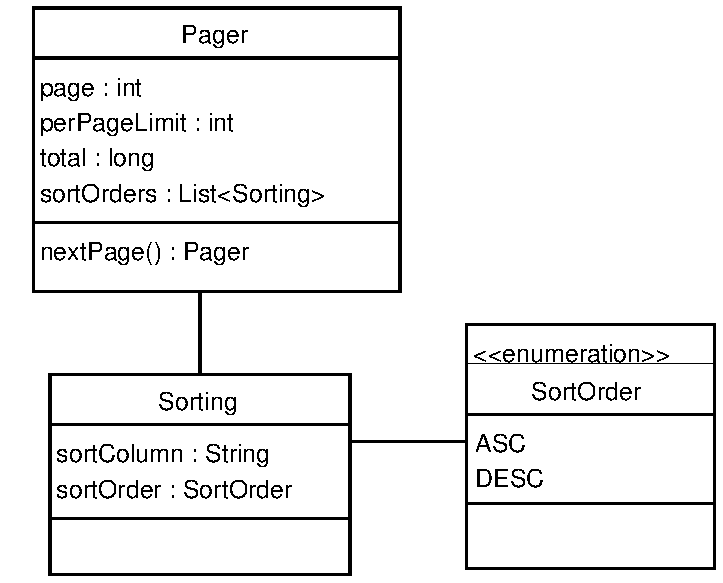
\includegraphics[width=0.7\linewidth]{images/pager_uml}}
	\caption{UML Diagramm der Paging Klassen}
\end{figure}

\subsection{Benutzerverwaltung}\label{service:security}
Da eine Anwendung fast ausnahmslos von mehreren Benutzern verwendet wird, müssen
sie in irgendeiner Form eindeutig identifizierbar sein. Auch hier stellt der Service
Layer wieder einen guten Ansatzpunkt dar, um die Aufgaben der Authentifizierung
und Autorisierung zu übernehmen.

\begin{description}
\item[Authentifizierung] Authentifizierung ist der Vorgang, einen Benutzer
eindeutig zu identifizieren und sicherzustellen, dass es sich um den
behaupteten Teilnehmer handelt. Grundsätzlich wird zwischen drei verschiedenen
Arten der Authentifizierung (vgl. \cite{kruth:2004} S. 295) unterschieden.
\begin{itemize}
\item Bei der Authentifizierung durch \emph{Wissen} handelt es sich
üblicherweise um die Kombination aus Benutzername und Passwort.
\item Ein Teilnehmer authentifiziert sich durch \emph{Besitz}, wenn er ein
Objekt mit den entsprechenden Authentizitätsinformationen besitzt,
beispielsweise eine Chipkarte.
\item Ferner ist es möglich, dass sich ein Teilnehmer durch
\emph{unveränderliche Eigenschaften}, wie zum Beispiel die biometrische
Eigenschaft eines Fingerabdrucks, authentifizieren kann.
\item Auch eine Kombination der verschiedenen Authentifizierungsmechanismen ist
möglich.
\end{itemize}
\item[Autorisierung] Berechtigungen werden von einem Administrator der Anwendung
vergeben und bestimmen, ob ein authentifizierter Teilnehmer auf bestimmte Domain
Objekte und Service Methoden zugreifen darf (vgl. \cite{kruth:2004} S. 292). Der
Vorgang der Überprüfung, ob ein Teilnehmer die benötigten Berechtigungen hat,
wird \emph{Autorisierung} genannt. Berechtigungen auf Domain Objekten hängen in den
meisten Fällen direkt mit den darauf auszuführenden \ac{CRUD} Operationen
zusammen. So dürfen manche Benutzer Domain Objekte lesen, erstellen und
verändern, während andere lediglich lesenden Zugriff darauf haben.
\end{description}

Die sichere Beschaffung und Übertragung der für die Authentifizierung eines
Benutzers notwendigen Informationen zum Service Layer ist weiterhin Aufgabe des
Benutzers.

\subsubsection{Spring Security}
Spring Security (vormals Acegi Security) ist ein Unterprojekt des Spring
Frameworks, das umfangreiche Möglichkeiten für die Authentifizierung
und Autorisierung von Benutzern bietet. Einige nennenswerte
Protokolle zur Benutzerauthentifizierung sind:

\begin{description}
	\item[LDAP] LDAP ist eine vor allem in großen Unternehmen häufig genutzte
	Möglichkeit, auf zentral gespeicherte Benutzerinformationen zugreifen zu
	können.
	\item[HTTP Authentifizierung] Auch die im \ac{HTTP} Protokoll
	spezifizierten Authentifizierungsmechanismen werden unterstützt.
	\item[OpenID] OpenID ist ein dezentralisierter, offener Standard für die
	Benutzerauthentifizierung. An einem Authentifizierungsvorgang beteiligt sind
	die Anwendung selbst, der zu authentifzierende Benutzer und ein OpenID
	Anbieter, bei dem der Benutzer seine Zugangsinformationen gespeichert hat.
	\item[UserService] Spring Security bietet auch die Möglichkeit, ein
	eigenes UserService Interface zu implementieren. Dadurch kann die Anwendung
	die für die Authentifizierung notwendigen Informationen selbst bereitstellen.
\end{description}

Hat sich ein Benutzer erfolgreich authentifiziert, legt Spring Security diese
Informationen in einem \emph{SecurityContext} ab, der dann in der gesamten
Anwendung verfügbar ist.

Ist der Context erstellt, also der Benutzer authentifiziert, bietet Spring
Security verschiedene Möglichkeiten zur Autorisierung der vom Benutzer
duchgeführten Aktionen. Unterstützt wird eine \emph{rollenbasierte
Authorisierung} (vgl. \cite{park:2001}), auf dessen Grundlage Service
Methoden oder einzelne Domain Objekte geschützt werden können. Die Grundidee der
rollenbasierten Authorisierung ist, dass Berechtigungen mit
Rollen\footnote{Mögliche Rollen sind beispielsweise Administrator, Manager, User
usw.} verbunden sind und den Benutzern dann diese Rollen zugewiesen werden.

\subsubsection{Implementierung}
Der Service zur Benutzerverwaltung übernimmt zwei Aufgaben. Zum Einen
die Administration von Benutzern und Rollen, zum Anderen die
Authentifizierung und Authorisierung eines Benutzers. Neben der Erstellung und
Implementierung des entsprechenden Service Interface ist es deshalb auch
notwendig, von \ac{GORM} verwaltete Domain Klassen für Benutzer und Rollen zu
erstellen. Abbildung \ref{ill:securitymodel} zeigt das entsprechende Domain
Model und die Interfaces, die aus dem Spring Security Framework verwendet
wurden.

\begin{figure}[bth]
    \center{\includegraphics[width=\linewidth]{images/securitymodel}}
	\caption{Benutzer und Rollen Domain Model mit Spring Security}
	\label{ill:securitymodel}
\end{figure}

Da der Service Layer unabhängig von seinen Benutzern als eigene Schicht arbeiten
soll, übernimmt er keine implementierungsspezifischen Aufgaben des verwendeten
Authentifizierungsmechanismus. Ist der Benutzer beispielsweise eine
Weboberfläche, muss die Umwandlung von der dort verwendeten \ac{HTTP} Authentifzierung in einen
Security Service Methodenaufruf bereits dort erfolgen. Abbildung
\ref{ill:securityservice} zeigt die Methoden des Security Service Interface.

\begin{figure}[bth]
    \center{\includegraphics[width=0.6\linewidth]{images/securityservice}}
	\caption{Security Service Interface}
	\label{ill:securityservice}
\end{figure}

\subsection{Logging und Monitoring}\label{service:logging}
Dadurch, dass eine Unternehmensanwendung von vielen Benutzern verwendet wird und
im Normalfall auch mit anderen entfernten Anwendungen kommuniziert, können
Fehler auftreten, die nicht immer direkt nachvollziehbar sind. Deshalb ist es
sinnvoll, den Programmablauf zu protokollieren, um Fehler leichter zu
lokalisieren und auch das Nutzungs- und Laufzeitverhalten besser nachvollziehen zu können. Dies wird
allgemein \emph{Logging} genannt. In lokalen Anwendungen können Debugger, die
eine Übersicht über den Zustand der Anwendung ermöglichen, für die Fehlersuche
verwendet werden. In verteilten Systemen, die über entfernte Methodenaufrufe
kommunizieren, ist diese Möglichkeit der Fehlersuche nicht mehr in dieser Form
realisierbar. Hier können aber Statusmeldungen durch Logging hilfreich sein, um
den Fehler auch in solchen Anwendungen besser eingrenzen zu können und die
Administratoren über aufgetretene Fehler zu informieren. Das Logging der
Ausführungszeiten einzelner Methoden kann außerdem dabei helfen die Laufzeit der
Anwendung zu optimieren. Auch die Auswertung des Benutzerverhaltens ist eine
wichtige Aufgabe des Loggings. Dadurch lassen sich Rückschlüsse führen
wie die Anwendung tatsächlich verwendet wird und verbessert werden kann.

Hinzu kommt der Trend, dass die Bezahlung für die Benutzung einer Anwendung
individuell nach dem tatsächlichen Nutzungsvolumen erfolgt (vgl.
\cite{brandon:2009}). Um dies zu ermöglichen bietet sich der zentrale Logging
Mechanismus ebenfalls an. Durch die Auswertung der protokollierten
Benutzeraktivitäten lässt sich dann eine nutzungsbezogene Rechnung stellen.

\subsubsection{Logging Frameworks für Java}
Es gibt eine Vielzahl an Logging Frameworks für Java, die aber meist ähnlichen
Ansätzen folgen. So werden mehrere Log Level\footnote{Üblich sind FATAL, ERROR,
WARN, INFO und DEBUG} unterstützt, für die Nachrichten bzw. Exception Objekte
protokolliert werden können. Auch ist es möglich, Logger an verschiedene
Ausgabesysteme anzubinden. Normalerweise handelt es sich dabei um eine Datei,
aber auch die Anbindung an eine Datenbank oder die Versendung von Nachrichten bei einem
bestimmten Log-Ereignis sind möglich. Idealerweise soll ein Framework nicht
direkt von der tatsächlichen Implementierung eines der vielen Java Logging
Frameworks abhängig sein, sondern diese Entscheidung dem Benutzer überlassen. Zu
diesem Zweck wurde das \ac{SLF4J}\footnote{\url{http://www.slf4j.org}}
entwickelt, das entsprechend dem \emph{Facade Design Pattern} ein Logging Interface bereitstellt und Methodenaufrufe an die
vom Benutzer gewählte Logging Implementierung weiterleitet.

\subsubsection{Implementierung}
Die Implementierung des Logging Service stellt grundsätzlich die Methoden dieses
Interfaces zur Verfügung. Zusätzlich wurde der Logging Mechanismus um sogenannte
\emph{Actions} erweitert. Diese repräsentieren jeweils Ereignisse, die ausgeführt
werden, sobald sie durch den Logging Service protokolliert werden. Dadurch kann
die unmittelbare Rechnungsstellung von Benutzeraktionen ebenso realisiert werden
wie die Ausführung von bestimmten Wiederherstellungsoperationen bei einem
kritischen Fehler. Zu Optimierung der Laufzeit können Log Meldungen und Actions
außerdem durch den verwendeten Cache Service gepuffert werden, um zu einem
späteren Zeitpunkt ausgeführt oder geschrieben zu werden.

\subsection{Internationalisierung}\label{service:i18n}
Hat die Anwendung eine sehr große Zahl an Anwendern, kann es vorkommen, dass eine
Anpassung an unterschiedliche Kulturzonen und Sprachen der Anwender benötigt
wird. Das ist vor allem bei öffentlich zugänglichen Webanwendungen der Fall, die
auf einen internationalen Markt abzielen. Die Erfahrung hat gezeigt, dass der
Aufwand für die Internationalisierung oft unterschätzt wird. Der Service Layer
als gemeinsame Anwendungsschnittstelle kann hierbei ein guter Ansatz sein, um
die Anwendung internationalisierbar zu machen und den damit verbundenen
Mehraufwand minimal zu halten.

\subsubsection{Internationalisierung in Java und Spring}
Bei der Übersetzung in andere Sprachen ist es üblich, Strings, die in
verschiedenen Sprachen vorkommen können, durch einen eindeutigen Schlüssel zu
ersetzen. Ist die gewünschte Sprache bekannt, wird dieser Schlüssel dann durch
den entsprechenden Sprachtext ersetzt. Für die Internationalisierung bieten die
Java Standardbibliothek und das Spring Framework verschiedene Klassen an, die die
Arbeit damit erleichtern:

\begin{description}
\item[Locale]
Locale\footnote{\url{http://java.sun.com/javase/6/docs/api/java/util/Locale.html}}
Objekte stellen eine geografische, politische oder kulturelle Region dar. Sie
werden entsprechend den ISO Abkürzungen für
Sprachen\footnote{\url{http://www.loc.gov/standards/iso639-2/englangn.html}} und
Länder\footnote{\url{http://www.iso.ch/iso/en/prods-services/iso3166ma/02iso-3166-code-lists/list-en1.html}}
repräsentiert. Operationen, die aufgrund des übergebenen Locale Objekts regions-
und sprachspezifische Ergebnisse zurückliefern, werden auch locale-sensitiv
genannt. Locale Objekte werden meist nicht instanziiert, sondern von der
\ac{JVM} bereitgestellt, die eine Liste der installierten Sprachen und den entsprechenden
Locale Objekten mitführt.
\item[Format]
Format\footnote{\url{http://java.sun.com/javase/6/docs/api/java/text/Format.html}}
ist eine abstrakte Basisklasse um locale-sensitive Informationen zu formatieren.
Für die gängigen Anwendungsfälle stellt die Java Standardbibliothek die
folgenden Implementierungen bereit:
\begin{itemize}
  \item \emph{DateFormat} für die Formatierung von Datumsangaben
  \item \emph{NumberFormat} für die Formatierung von Zahlen unter
  Berücksichtigung der für die Locale üblichen Trennzeichen
  \item \emph{MessageFormat} um Nachrichten sprachunabhängig zusammenzusetzen
  und dann entsprechend einer \emph{Locale} zu formatieren
\end{itemize}
\item[ResourceBundle] Ein
ResourceBundle\footnote{\url{http://java.sun.com/javase/6/docs/api/java/util/ResourceBundle.html}}
ist eine abstrakte Basisklasse, die lokalisierte Objekte bereitstellt. Auf die
Objekte kann über die Kombination aus einem eindeutigen String (Schlüssel) und
dem Locale Objekt für die gewünschte Sprache zugegriffen werden.
\item[MessageSource] Eine
MessageSource\footnote{\url{http://static.springsource.org/spring/docs/3.0.x/javadoc-api/org/springframework/context/MessageSource.html}}
ist ein vom Spring Framework zur Verfügung gestelltes Interface, das den Zugriff
auf internationalisierte Nachrichten vereinfacht. Die bereitgestellten
Implementierungen verwenden das oben beschriebene \emph{ResourceBundle} um die
Nachrichten aufzulösen und das entsprechende \emph{MessageFormat} um diese zu
parameterisieren.
\end{description}

In der Standardimplementierung benutzt ein \emph{ResourceBundle} die von Java
unterstützten \emph{Property} Dateien. Für jeweils eine unterstützte Locale wird
eine Datei angelegt, die als Konvention das Kürzel der entsprechenden Locale am
Ende des Dateinamens enthält. In dieser Datei erfolgt dann die Zuordnung von
einem Schlüssel zu der passenden Übersetzung mit Platzhaltern für Inhalte, die
dynamisch eingefügt werden. Listing \ref{lst:i18nprops} zeigt ein entsprechendes Beispiel.

\lstset{language=Python}
\lstinputlisting[caption=Beispiel für die Internationalisierung mit
Properties, label=lst:i18nprops] {sources/i18n_examples.properties}

\subsubsection{Implementierung}
Das Interface des I18n\footnote{I18n ist die allgemein verwendete Abkürzung für
\emph{Internationalization}, weil zwischen dem ersten und letzten Buchstaben 18
weitere Buchstaben stehen} Service fasst nun die Schnittstellen der oben
vorgestellten Klassen zusammen und bindet sie in das Gesamtkonzept des Service
Layer ein.

\begin{figure}[bth]
    \center{\includegraphics[width=\linewidth]{images/i18nservice}}
	\caption{Interface und Domain Klassen des I18n Service}
	\label{ill:i18nservice}
\end{figure}

So ist es möglich, in Verbindung mit dem Security Service die bevorzugte
Locale eines Benutzers zu bestimmen. Diese Information kann entweder bereits
beim Anlegen eines Benutzers gespeichert werden oder dynamisch in der über dem
Service Layer liegenden Schicht bestimmt werden, beispielsweise durch die Liste
der bevorzugten Sprachen im Header einer \ac{HTTP} Anfrage.

Wenn sich die Inhalte der übersetzten Texte häufig ändern kann es sehr unflexibel
sein, diese in Java Property Dateien zu speichern, da man direkten Zugriff auf
das Dateisystem benötigt. Deshalb unterstützt der I18N Service auch eine Domain
Klasse zur Speicherung von Übersetzungstexten, die über den Domain Model Service
in der Datenbank gespeichert wird. Damit ist es deutlich einfacher möglich,
diese Texte zu aktualisieren, beispielsweise über das Administrationsmenü der
Anwendung. Abbildung \ref{ill:i18nservice} zeigt das Service Interface und die
Domain Klasse für Übersetzungstexte. Da auch die Übersetzungen über einen
eindeutigen Schlüssel zugeordnet werden und sich relativ selten ändern, eignet
sich der Cache Service sehr gut um diese für einen schnellen Zugriff zu
speichern.
\myChapter{Remoting Layer}\label{chap:remotinglayer}
Eine besondere Form des Presentation Layer ist der Remoting Layer, der die
Aufgabe übernimmt eine Anwendung über verscheidene \ac{RPC} Protokolle
anzubinden. In diesem Kapitel soll zuerst ein zentralisierter
Ausführungsmechanismus vorgestellt werden, der eine verallgemeinerte Form eines
\ac{RPC} Aufrufs annehmen kann. Anschließend werden konkrete \ac{RPC} Protokolle
und deren Implementierungen besprochen, die einen Aufruf in diese Form umwandeln
können.

\section{Service Engine}\label{sec:serviceengine}
Im Service Layer werden eine Reihe von Java Interfaces bereitgestellt, welche die
nach außen hin sichtbare Schnittstelle einer Anwendung definieren. Da die Service
Methoden so kompakt wie möglich gehalten werden sollten und nur die Methoden
bereitgestellt werden, die auch tatsächlich von den Benutzern verwendet werden,
eignen sich diese Interfaces auch als Schnittstelle für entfernte Methodenaufrufe
(vgl. \cite{fowler:2002} S. 135).

Zu diesem Zweck existieren in Java eine Reihe von Bibliotheken, die verschiedene
\ac{RPC} Protokolle implementieren. Jede Bibliothek verfolgt dabei ein eigenes
Konzept, wie ein Service in dem entsprechendem \ac{RPC} Protokoll zur Verfügung
gestellt wird. Möchte man eine Schnittstelle über verschiedene Protokolle zur
Verfügung stellen ist es notwendig, jede Bibliothek individuell zu
konfigurieren, obwohl die dafür notwendigen Informationen jeweils identisch sind. Gleichzeitig
fehlt ein zentraler Ausführungsmechanismus, da jede \ac{RPC} Bibliothek die
Ausführung der aufgerufenen Methoden selbst übernimmt.

Diesen Nachteilen soll die Zwischenschicht der Service Engine entgegenwirken,
indem sie die Verwaltung aller vorhandenen Services und die zentrale Ausführung
von Methoden übernimmt, ohne selbst ein \ac{RPC} Protokoll zu implementieren.
Implementierungen eines Protokolls (anschließend \emph{Protocol Handler} genannt)
sind dann die der Service Engine übergeordneten Schichten. Sie müssen lediglich
die Konvertierung eines konkreten \ac{RPC} in eine allgemeine Form übernehmen, die
dann an die Service Engine zur Ausführung übergeben werden kann.

Einzuordnen ist die Service Engine als Zwischenschicht direkt über dem Service
Layer, befindet sich aber bereits in der vormals eingeführten Remoting Schicht
(siehe Abbildung \ref{ill:serviceengine}).

\begin{figure}[bth]
    \center{\includegraphics[width=\linewidth]{images/overviews/serviceengine}}
	\caption{Einordnung der Service Engine}
	\label{ill:serviceengine}
\end{figure}

\subsection{Remote Schnittstelle}
Das Konzept des Service Layer sieht vor, dass sich die Service Methoden direkt
nach den Anforderungen der Benutzer richten. Als direkt übergeordnete Schicht ist
auch die Service Engine ein Benutzer des Service Layer und kann deshalb ebenfalls
auf die Erstellung der Service Layer Schnittstelle Einfluss nehmen. Dabei
richten sich die Anforderungen der Service Engine wiederum nach den Protocol
Handlern und den \ac{RPC} Protokollen, die diese implementieren. Obwohl der
Service Layer keine direkten Abhängigkeiten von seinen übergeordneten Schichten
haben sollte, wirken sich die unterstützten \ac{RPC} Protokolle somit trotzdem
indirekt auf die Implementierung des Service Layer aus.

Nicht alle \ac{RPC} Protokolle stellen dabei den gleichen Funktionsumfang zur
Verfügung. Das erste wichtige Unterscheidungsmerkmal ist, ob ein \ac{RPC} mit
Objekten und Methodenaufrufen arbeitet oder einfache Prozeduraufrufe übertragen
werden. Im letzteren Fall muss der Service Layer entsprechend so gestaltet
werden, dass die einzelnen Service Methoden wie getrennte Prozeduren ausgeführt werden
können, die nicht zu einem Objekt gehören. Ein weiterer zu beachtender Punkt ist,
ob ein \ac{RPC} Protokoll zustandsgebunden oder zustandslos arbeitet.
Zustandsgebunden heißt auch, dass ein Client über verschiedene Anfragen das
gleiche Service Objekt zur Verfügung hat, während bei einem zustandslosen Protokoll jede
Anfrage unabhängig von allen anderen Anfragen und ohne einen globalen Zustand
bearbeitet wird\footnote{Das bedeutet normalerweise, dass für jede Anfrage ein
neues Service Objekt erzeugt wird}.

Bei dem Entwurf und der Implementierung der Service Interfaces, die über die
Service Engine angebunden werden sollen, muss also der "`kleinste gemeinsame
Nenner"' zwischen den anzubietenden \ac{RPC} Protokollen gefunden werden. In
Abschnitt \ref{sec:protocolhandler} werden diese Einschränkungen an den dort
vorgestellten \ac{RPC} Protokollen näher analysiert.

\subsection{Service Registry}
Der zentrale Bestandteil der Service Engine ist das Interface der \emph{Service
Regitry}. Die Service Registry übernimmt die Verwaltung der Service Interfaces,
die Instanziierung entsprechender Objekte, sowie die zentrale Ausführung von
Methoden auf diesen Objekten. Jedem Service Interface ist hierbei ein eindeutiger
Name zugewiesen. Wie die Services verwaltet und instanziiert werden, bleibt
dabei der Klasse überlassen, die das Service Registry Interface implementiert. 

Da andere Teile der Implementierung bereits auf dem Spring Framework basieren,
hat es sich angeboten eine Service Registry zu implementieren, die auf dem
\emph{Application Context} des Dependency Injection Containers basiert. Die
Instanziierung und Benennung von Service Objekten wird hier bereits bei der
Erstellung des Spring Context vorgenommen. Die Implementierung des Service
Registry Interface in Form der \emph{ApplicationContextRegistry} stellt nun alle
Objekte aus einem Application Context als Service Objekte bereit, sofern sie nach
einer festgelegten Namenskonvention benannt sind. In der Standardeinstellung
werden alle Objekte, deren Name auf "`Service"' endet, über die Service Registry
verfügbar gemacht. Da diese Endung in der Service Registry eine redundante
Information darstellen würde, wird sie entfernt um daraus den eindeutigen Namen
für den bereitgestellten Service zu generieren. Beispielsweise ist das Context
Objekt "`userService"' dann in der Service Registry unter dem Namen "`user"'
verfügbar. Die Zuordnung von Objekten aus dem Application Context zu einem
Service Interface muss manuell vorgenommen werden, da ein Objekt auch mehrere
Service Interfaces implementieren kann. Die für die Ausführung von Methoden
wichtigen Bestandteile der Service Registry sollen in den folgenden Abschnitten
näher erläutert werden.

\subsection{Interne RPC Darstellung}
Wie bereits erwähnt ist es nicht die Aufgabe der Service Engine, ein konkretes
\ac{RPC} Protokoll zu implementieren. Das bedeutet, dass die übergeordnete
Schicht der Service Engine einen Methodenaufruf in einer verallgemeinerten Form
zur Verfügung stellen muss. Da diese Schicht in erster Linie aus
verschiedenen \ac{RPC} Protocol Handlern besteht, die ebenfalls in Java
implementiert werden, bietet sich für die allgemeine Darstellungsform eines Methodenaufrufs
deshalb die Implementierung einer entsprechenden Java Klasse an. Diese Klasse
muss alle Informationen enthalten, die für die Ausführung
benötigt werden:

\begin{itemize}
  \item Den Namen des Service in der Service Registry
  \item Den Namen der aufzurufenden Methode
  \item Eine Liste der Methodenparameter
  \item Eine Liste der Parameter Typen
  \item Informationen über den serverseitigen Zustand des Client
\end{itemize}

In Java lässt sich der Typ eines Parameters zur Laufzeit anhand der Instanz des
Parameter Objekts bestimmten, muss deshalb also nicht getrennt gespeichert
werden. Der serverseitige Zustand eines Client wird im folgenden Abschnitt näher
behandelt.

Die \emph{RemoteProcedureCall} Klasse wurde als unveränderliches Klasse mit den
oben genannten Datenelementen implementiert. Ein RemoteProcedureCall Objekt dient
lediglich als Transferobjekt zwischen der Service Engine und der übergeordneten
Schicht. Die Validierung und eventuell
notwendige Konvertierung von Parametern erfolgt dann an zentraler Stelle in der
Service Registry und wird in Abschnitt \ref{subsec:dispatcher} genauer
betrachtet.

\subsection{Sessions}\label{subsec:sessions}
Bei einem \ac{RPC} wird zwischen zustandslosen und zustandsbehafteten Protokollen
unterschieden, was auch bei der Ausführung von Methoden in der Service Registry
beachtet werden muss. Für die zustandslose Kommunikation kann für jede Anfrage
auf der Service Registry ein neues Service Objekt erstellt werden, auf dem die
übergebene Methode ausgeführt wird. Im Gegensatz dazu muss sich ein Client bei
einer zustandsbehafteten Kommunikation zu Beginn bei dem Server authentifizieren.
Nach einer erfolgreichen Authentifizierung kann der Server alle nachfolgende
Anfragen des Client diesem wieder eindeutig zuordnen. Das bedeutet auch, dass der
Client üblicherweise erwartet, für alle folgenden Anfragen die jeweils gleiche
Instanz eines Service Objekts zur Verfügung zu haben. Der serverseitige Zustand
von Objekten, die über die zustandsgebundene Kommunikation einem einzigen Client
zugeordnet sind, soll nachfolgend \emph{Session} genannt werden.

Wie für die allgemeine Form eines \ac{RPC} die RemoteProcedureCall Klasse
entwickelt wurde, ist es auch für Sessions notwendig einen Ansatz zu
implementieren, der unabhängig von einem bestimmten \ac{RPC} Protokoll arbeitet.
Da die Umsetzung von Sessions in verschiedenen Protokollen unterschiedlich
gehandhabt wird, bleibt die Erstellung und Zuordnung einer Session dem jeweiligen
Protocol Handler überlassen, während die Verwaltung an zentraler Stelle in der
Service Registry erfolgt. Ein Session Objekt repräsentiert jeweils den
serverseitigen Zustand eines bestimmten Clients. Zur Zuordnung und Identifikation
besitzt jedes Session Objekt einen eindeutigen Bezeichner (\emph{Session ID}).
Aufgabe des Protocol Handler ist es nun, Anfragen eines Client mit der
entsprechenden Session ID zu verbinden, so dass die Service Registry den
korrekten serverseitigen Zustand für die Ausführung der Anfrage auswählen
kann.

Auch für die Implementierung von Sessions bietet das Spring Framework eine gute
Grundlage. Bei der Definition eines Objekts im Context kann angegeben werden,
über welchen Zeitraum (\emph{Scope}) eine Objektinstanz im Application Context
zur Verfügung stehen soll. Standardmäßig unterscheidet Spring hierbei zwischen
\emph{Singleton} und \emph{Prototype}. Ein Singleton Objekt wird bei der
Initialisierung des Application Context erstellt und ist über die gesamte
Laufzeit der Anwendung verfügbar. Wird eine Referenz auf das Objekt angefordert
handelt es sich also immer um die gleiche Instanz. Im Gegensatz dazu wird ein
Prototype Objekt für jede angeforderte Referenz neu erstellt. Durch die hohe
Flexibilität des Spring Frameworks ist es auch möglich eigene Scopes für
Objekte zu definieren. Diese Möglichkeit wurde bei der Implementierung
verwendet um einen Scope zu erstellen, der an jeweils ein Session Objekt der
Service Registry gebunden ist. Möchte man also ein Objekt aus dem Spring
Context für jeweils einen Benutzer verfügbar machen, muss es im Context mit
diesem Scope definiert werden.

\subsection{Methodenausführung}\label{subsec:dispatcher}
Nachdem nun ein allgemeines Transferobjekt für einen \ac{RPC} in Form der
RemoteProcedureCall Klasse implementiert wurde und auch zustandsgebundene
Protokolle mit Hilfe der Session Umgebung in der Service Engine einen
serverseitigen Zustand erhalten, ist die Service Registry nun in der Lage,
die Informationen aus einem RemoteProcedureCall Objekt in einen Methodenaufruf
auf einem Service Objekt umzusetzen.

Den Benutzern der Service Engine werden bei der Erstellung eines passenden
RemoteProcedureCall Objekts bewusst verschiedene Möglichkeiten gegeben, in
welcher Form die Methodenparameter übergeben werden können. Dadurch ist die
Verwendung der Service Engine weniger komplex und die Konvertierung und
Validierung von Parametern erfolgt an zentraler Stelle in der Service Registry.
Eine wichtige Rolle spielt dabei die in Kapitel \ref{subsec:assocequ} behandelte
Äquivalenz zwischen JavaBeans und Assoziativen Arrays. Viele \ac{RPC} Protokolle
benutzen für die Übertragung von Objekten ein Format, dass sich relativ leicht in
ein assoziatives Array (Map) deserialisieren lässt\footnote{Beispielsweise
\ac{JSON}}. Damit nicht jeder Protocol Handler die Umwandlung in ein passendes
JavaBean selbst übernehmen muss, wird die Konvertierung von einem assoziativen
Array in ein JavaBean von der Service Registry vorgenommen. Hierfür wurde
ein Algorithmus implementiert, der bei einem gegebenen assoziativen Array aus
einer Reihe von JavaBean Klassen die passendste Implementierung auswählt, diese
instanziiert und die Properties des JavaBean mit den entsprechenden Werten der
Map füllt. Die ausgewählte JavaBean Klasse ist diejenige, deren Eigenschaften
am genauesten mit den Schlüsseln der übergebenen Map übereinstimmen. Für die
Suche der auszuführenden Methode ergibts sich dann das folgende Vorgehen:

\begin{enumerate}
  \item Im ersten Schritt muss das Service Objekt bestimmt werden. Über den
  Namen des Service wird es entweder in der Service Registry neu erstellt oder,
  wenn eine Session Umgebung vorliegt und das Objekt mit dem gegebenen Namen
  dort vorhanden ist, aus einer Session geholt.
  \item Daraufhin wird überprüft, ob das Service Interface eine Methode
  besitzt, die bereits mit dem Namen und der exakten Signatur des übergebenen
  RemoteProcedureCall Objekts übereinstimmt. Aufgrund einer Beschränkung in der
  Java Reflection muss Polymorphie bei den Parametern manuell geprüft
  werden\footnote{\url{http://stackoverflow.com/questions/2169497/unexpected-class-getmethod-behaviour}}.
  Wurde eine Methode gefunden, wird sie auf dem Service Objekt ausgeführt. 
  \item Wurde keine passende Methode gefunden, werden alle Methoden mit dem
  Namen und der Anzahl von Parametern des RemoteProcedureCall Objekts gesucht.
  Nun wird für jeden Parameter überprüft, ob es sich um ein assoziatives Array
  handelt. Ist dies der Fall, wird unter allen Parameter Typen der Methoden an
  dieser Stelle das passendste JavaBean instanziiert. Mit diesen neu gewonnenen
  Parametern wird nun erneut Schritt zwei ausgeführt.
  \item Wurde keine Methode gefunden, wird eine NoSuchMethodError Exception
  geworfen. Als Erweiterung der Ausführungsvorgangs hat ein Service Objekt noch die
  Möglichkeit grundsätzlich alle Methodenaufrufe behandeln zu können, indem es
  das \emph{Interceptable} Interface implementiert. Wurde in den Schritten zwei
  und drei keine passende Methode gefunden, wird der Methodenaufruf an dieses
  Interface übergeben.
\end{enumerate}

\subsection{Übersicht}
Das \ac{UML} Diagramm in Abbildung \ref{ill:serviceengine_uml} zeigt die
wichtigsten an der Service Engine beteiligten Interfaces. Die Schnittstelle der
Service Engine zu übergeordneten Schichten besteht aus dem ServiceRegistry und
dem Session Interface sowie der RemoteProcedureCall Klasse. Das ProtocolHandler
Interface wird von Klassen implementiert, die eine Instanz einer Service Registry
benötigen.

\begin{figure}[bth]
    \center{\includegraphics[width=\linewidth]{images/uml/serviceengine}}
	\caption{UML Diagramm der wichtigsten Komponenten der Service Engine}
	\label{ill:serviceengine_uml}
\end{figure}

\pagebreak
\section{Protocol Handler}\label{sec:protocolhandler}
Die Service Engine stellt über die Schnittstelle der Service Registry eine
Möglichkeit zur Verfügung, einen \ac{RPC} in der allgemeinen Form des
\emph{RemoteProcedureCall} Objekts ausführen zu können. Es ist nun die Aufgabe
der \emph{Protocol Handler}, die tatsächliche Implementierung der verschiedenen
\ac{RPC} Protokolle bereitzustellen und der Service Registry in Form dieses
Objekts zur Ausführung zu übergeben. Die Aufgaben eines Protocol Handler umfassen
somit:

\begin{itemize}
  \item Beschreibung der Java Interfaces in der \ac{IDL} des
  implementierten \ac{RPC} Protokolls, soweit notwendig. Für die meisten
  \ac{RPC} Protokolle beinhaltet das Java Service Interface bereits alle
  Informationen, die für die Schnittstellenbeschreibung notwendig sind.
  \item Bereitstellung eines Namensdienstes zur Auffindung der Services
  einer Service Registry, soweit nowendig.
  \item Annahme von Anfragen in einem spezifischen \ac{RPC} Protokoll.
  \item Initialisierung einer zu dem \ac{RPC} Protokoll gehörigen Session
  Umgebung.
  \item Deserialisierung von Methodenaufrufen und Umwandlung in ein
  RemoteProcedureCall Objekt.
  \item Übergabe des RemoteProcedureCall Objekts an die Service Registry zur
  Ausführung des Methodenaufrufs.
  \item Serialisierung des Ergebnisses in das Austauschformat des \ac{RPC}
  Protokolls und Übertragung dieser Daten.
  \item Serialisierung von Fehlern, die während der Methodenausführung
  aufgetreten sind.
\end{itemize}

In der Gesamtarchitektur sind die Protocol Handler im Remoting Layer über der
Service Engine einzuordnen (siehe Abbildung \ref{ill:protocolhandler}). Es ist
die Schicht des Gesamtsystems, mit der andere entfernte System direkt
kommunizieren.

\begin{figure}[bth]
    \center{\includegraphics[width=\linewidth]{images/overviews/protocolhandler}}
	\caption{Einordnung der Protocol Handler}
	\label{ill:protocolhandler}
\end{figure}

Es ist weiterhin möglich, die Implementierungen vorhandener \ac{RPC} Protokolle
zu verwenden, so lange die Möglichkeit besteht, Methodenaufrufe in die
abstrahierte Form des RemoteProcedureCall Objekts zu konvertieren und an die Service Registry
zu übergeben. In diesem Kapitel sollen drei unterschiedliche \ac{RPC} Protokolle
und deren Implementierungen eines Protocol Handler vorgestellt werden. Die
ausgewählten Protokolle verfolgen jeweils unterschiedliche Ansätze bezüglich
serverseitigem Zustand und der Art von Methoden- bzw. Prozeduraufrufen. Deshalb
sind sie gut geeignet, die Vorteile, die durch die Verwendung der Service Engine
entstehen, aufzuzeigen.

\subsection{Remote Method Invocation}\label{subsec:rmi}
Java \ac{RMI} (siehe \cite{sun:rmi}) ist die Implementierung eines binären
\ac{RPC} Protokolls für den Austausch von Objekten zwischen verschiedenen, auch
entfernten, Instanzen einer \ac{JVM}. Es setzt dabei stark auf die von der
\ac{JVM} unterstützten Serialisierung von Objekten. \ac{RMI} ist
zustandsgebunden, wodurch auch auf entfernten Objekten Methodenaufrufe
ausgeführt werden können. An der für \ac{RMI} notwendigen Infrastruktur sind
folgende Komponenten beteiligt (siehe \cite{wiki:rmi}):

\begin{description}
\item[Remote Interface] Das Remote Interface ist ein Java Interface, das dem
Client bekannt ist und die auf dem Server implementierten Methoden beschreibt.
Dadurch wird das Problem, die vom Server bereitgestellten Methoden zu
beschreiben, auf eine für Java natürliche Art und Weise gelöst.
\item[Remote Object] Das Remote Object ist eine Instanz der Klasse, die das
Remote Interface auf der Serverseite implementiert.
\item[RMI Registry] Die \ac{RMI} Registry ist ein Namensdienst, der für das
Auffinden der vom Server bereitgestellten Remote Objekte zuständig ist. Jeweils
einem implementierten Remote Interface wird dabei ein eindeutiger Name
zugewiesen.
\item[Remote Reference] Erkundigt sich der Client bei der \ac{RMI} Registry nach
dem Remote Object für einen bestimmten Namen, bekommt er eine Referenz auf das
serverseitige Remote Object zurück.
\end{description}

Ist die Verbindung von einem Client zu einem Remote Object auf dem Server
hergestellt, erlaubt \ac{RMI} eine transparente Kommunikation. Auch
Klassendefinitionen, die auf der jeweils anderen Teilnehmerseite nicht
vorhanden sind, werden dynamisch nachgeladen. Tritt einer der bei einem
\ac{RPC} zusätzlichen Fehlerfälle auf, wird eine \emph{RemoteException}
geworfen. Abbildung \ref{ill:rmi} zeigt den Ablauf der \ac{RMI}
Kommunikation und den beteiligten Komponenten.

\begin{figure}[bth]
	\center{\includegraphics[width=\linewidth]{images/rmischema}}
	\captionof{figure}[RMI Kommunikation]{Kommunkationsablauf bei
	RMI\footnotemark}
	\label{ill:rmi}
\end{figure}
\footnotetext{Quelle: \cite{wiki:rmi}, Public Domain}

\subsubsection{Spring und RMI}
Das Spring Framework vereinfacht die Nutzung von \ac{RMI} erheblich (vgl.
\cite{spring:reference} Abschnitt 19.2). So können in einem Kontext definierte
Objekte ebenfalls über eine Context Konfiguration als \ac{RMI} Services
exportiert werden, wenn sie das zu exportierende Remote Interface implementieren.

Da das Spring Framework durch Dependency Injection bereits die Verwendung von
Interfaces unterstützt, muss im Spring Context der Clientseite dann lediglich
ein \emph{Proxy} definiert werden, der das Remote Interface für den Client
implementiert und mit dem im Context angegeben \ac{RMI} Server
kommuniziert. Für Klassen des Client, die das Remote Interface verwenden, wird
dann dieser Proxy injiziert.

Listings \ref{lst:rmiserver} und \ref{lst:rmiclient} zeigen eine Spring Context
Konfiguration für die Verwendung des in Abschnitt \ref{service:i18n}
vorgestellten I18NService über \ac{RMI}.

\lstset{language=xml}
\lstinputlisting[caption=Spring und RMI - Server Context,
label=lst:rmiserver]{sources/springrmiserver.xml}

\lstinputlisting[caption=Spring und RMI - Client Context,
label=lst:rmiclient]{sources/springrmiclient.xml}

\subsubsection{Implementierung}
Da Spring bereits eine sehr gute Unterstützung für \ac{RMI} besitzt ist es
sinnvoll die dafür verwendeten Klassen für die Implementierung eines \ac{RMI}
Protocol Handler zu erweitern. Die \emph{RmiProtocolHandler} Klasse erstellt so für jeden
in der Service Registry vorhandenen Service eine Instanz des Spring
\emph{RmiServiceExporter} mit den passenden Parametern für Service Name, Service
Instanz und Service Interface. Dadurch sind bereits alle Service Interfaces über
\ac{RMI} auffindbar.

Schwieriger gestaltet sich nun die Bereitstellung des passenden Remote Object.
Der Client ruft über das ihm bekannte Remote Interface eine Methode auf einem
serverseitigen Remote Object auf. Auf dem Remote Object selbst verhält sich
dieser Aufruf genauso wie ein lokaler Methodenaufruf. Die Aufgabe des Protocol
Handler ist es aber, diesen Aufruf in ein entsprechendes
\emph{RemoteProcedureCall} Objekt umzuwandeln. Um diese Umwandlung zu
realisieren, wird ein Service Interface von einem \ac{AOP} Proxy\footnote{Siehe Abschnitt
\ref{define:aop}} implementiert, der dann als Remote Object dient. Durch einen
\emph{Around Advice} für alle Methodenaufrufe auf diesem Proxy ist es nun
möglich, die Informationen des Methodenaufrufs zu extrahieren und in ein
\emph{RemoteProcedureCall} Objekt umzuwandeln, das dann an die Service Registry
übergeben werden kann. Auch die Identifikation der Session ist bei diesem
Vorgehen problemlos möglich, da ein Remote Object, also hier das Proxy Objekt,
immer direkt einem Client zugeordnet ist.

\subsection{XML-RPC}\label{subsec:xmlrpc}
XML-RPC ist ein zustandsloses \ac{RPC} Protokoll, das \ac{XML} als
Austauschformat und \ac{HTTP} als Übertragungsprotokoll verwendet (siehe
\cite{winer:1999}). Übertragen werden Prozeduraufrufe, wobei die Struktur bewusst
sehr einfach gehalten wird, weshalb das Protokoll sowohl auf Server- als auch auf
Clientseite leicht zu implementieren ist.

\subsubsection{Spezifikation}
Als Parameter- und Rückgabewerte werden sieben primitive und zwei
zusammengesetzte Typen unterstützt. Ein Typ wird jeweils von einem \emph{<value>}
XML Tag umschlossen. Die primitiven XML-RPC Typen sind in Tabelle
\ref{tab:xmlrpcprimitives} aufgelistet. Der zusammengesetzte Typ \emph{Struct}
ist das XML-RPC Äquivalent eines assoziativen Arrays, während der Typ
\emph{Array} eine geordnete Menge von beliebigen anderen XML-RPC Typen enthält. Im Fehlerfall
wird ein \emph{Fault} Objekt übertragen, das ein Struct Element mit den
Schlüsseln \emph{faultCode} und \emph{faultString} enthält.


\begin{table}[h] \begin{tabularx}{\textwidth}{lll} \toprule
   \tableheadline{Typ} & \tableheadline{XML Tag} &
    	\tableheadline{Beispiel} \\
   		\midrule Integer & <i4> oder <int> & <int>33</int>\footnotemark \\
    	Double & <double> & 3.1415 \\
    	Date/Time & <dateTime.iso8601> & 20100223T19:34:56 \\
    	Boolean & <boolean> & 1, 0, true, false \\ 
    	String & <string> & Text \\
    	Base64 Binärdaten & <base64> & VGV4dA== \\
		\bottomrule
	\end{tabularx}
\caption[XML-RPC primitive Typen]{Primitive Typen des XML-RPC Protokolls}
\label{tab:xmlrpcprimitives}
\end{table}
\footnotetext{In den weiteren Beispielen wurden die umschließenden XML Tags aus
Platzgründen weg gelassen}

Da XML-RPC \ac{HTTP} als Übertragungsprotokoll verwendet, erfolgt die
Lokalisierung über einen eindeutigen \ac{HTTP} \ac{URI}, wohin alle
Prozeduraufrufe gerichtet werden. Die XML-RPC Spezifikation sieht nicht vor, die zur Verfügung gestellten
Prozeduren automatisch zu beschreiben. Die Beschreibung erfolgt meist in Form
einer \ac{API} Dokumentation. Eine inoffizielle aber häufig verwendete
Erweiterung zur Schnittstellen Beschreibung ist die \emph{XML-RPC Introspection}
(siehe \cite{henderson:2007}).

Ein vollständiges Beispiel einer XML-RPC Kommunikation mit dem Aufbau von Struct,
Array und Fault Elementen sowie den dazugehörigen \ac{HTTP} Headern ist in
Anhang \ref{chap:appendix} zu finden.

\subsubsection{Implementierung}
Für Java existieren eine Reihe von Bibliotheken, die XML-RPC Anfragen verarbeiten
können. Deshalb bot es sich, an eine passende Implementierung für die Umsetzung
des XML-RPC Protocol Handler zu verwenden. Voraussetzung ist, dass die
Bibliothek die Möglichkeit bietet, eine eigene Implementierung für die
Bearbeitung eines deserialisierten XML-RPC zur Verfügung zu stellen. Nach der Evaluierung
verschiedener Bibliotheken fiel die Entscheidung dabei auf die \emph{Redstone
XML-RPC Library}\footnote{\url{http://xmlrpc.sourceforge.net/}}, da sie
performant arbeitet, klar strukturiert ist und eigene Erweiterungen zulässt. Für
die Realisierung musste dann lediglich ein Interface implementiert werden,
das bei einem XML-RPC Aufruf mit den entsprechenden Methodennamen und
Parametern aufgerufen wird. Dort wird dann das entsprechende
RemoteProcedureCall Objekt erstellt und an die Service Registry weitergegeben.

\subsection{Representational State Transfer}\label{subsec:rest}
Der Begriff \ac{REST} wurde von Roy T. Fielding im Jahr 2000 in
\cite{fielding:2000} (S. 76 - 106) geprägt und beschreibt einen Software
Architekturstil für verteilte Hypermedia Systeme. Hypermedia (vgl.
\cite{fielding:2000} S. 68) bedeutet die Verwendung von
\emph{Multimedia-Formaten} und \emph{Hypertext}\footnote{Beispielsweise in Form
von HTML oder XML} zur Übertragung von Informationen, wobei in einem
Hypertext-Dokument wiederum durch \emph{Hyperlinks} auf andere Hypermedia Inhalte
verwiesen werden kann. Verteilte Hypermedia Systeme erlauben es, diese Inhalte
auch von einem entfernten System zu beziehen.

Bei \ac{REST} handelt es sich um einen Architekturstil, also eine Richtlinie,
wie Anwendungen, die die für \ac{REST} festgelegten Kriterien erfüllen, strukturiert
werden können. Somit ist \ac{REST} selbst implementierungs- und
technologieunabhängig. Das bekannteste Beispiel einer Umsetzung des \ac{REST}
Architekturstils ist das \ac{HTTP} Protokoll, das im nachfolgenden Abschnitt
genauer behandelt wird. Anwendungen, die der \ac{REST} Architektur folgen,
werden auch als \emph{RESTful} bezeichnet. Damit eine Implementierung dem
\ac{REST} Architekturstil, folgt stellt Fielding verschiedene Bedingungen auf
(siehe \cite{fielding:2000} S. 76 - 85):

\begin{description}
  \item[Client-Server] Durch die Verwendung einer Client-Server Architektur ist
  eine einfache Trennung der Aufgabenbereiche (\emph{Separation Of Concerns}) für
  beide Teilnehmer möglich. Dabei ist der Client für die Darstellung zuständig,
  während der Server die Datenhaltung und die Anwendungslogik übernimmt.
  Verschiedene Clients können dabei die vom Server bereitgestellten Daten in
  unterschiedlichen Benutzeroberflächen bereitstellen und verarbeiten, während
  die serverseitige Anwendungslogik gleichzeitig vereinfacht werden kann. Ein
  weiterer Vorteil ist, dass beide Seiten unabhängig voneinander weiterentwickelt
  werden können, so lange sie das entsprechende Protokoll und Austauschformat
  einhalten.
  \item[Zustandslosigkeit] Die Kommunikation zwischen Client und Server erfolgt
  zustandslos. Das heißt, dass ein Client mit jeder Anfrage alle für die
  Bearbeitung der Anfrage notwendigen Informationen übertragen muss. Dadurch
  verringert sich die Komplexität der Serverseite weiter, da jede Anfrage
  unabhängig von einem globalen Zustand bearbeitet werden kann. Gleichzeitig
  wird die Skalierbarkeit erhöht, da jede Anfrage von einer beliebigen
  Serverinstanz bearbeitet werden kann.
  \item[Cache] Im Hinblick auf die Netzwerkauslastung kann sich eine zustandslose
  Kommunikation negativ auswirken, da viele Informationen mehrfach übertragen
  werden müssen. Deshalb sieht \ac{REST} die Verwendung von Caches vor. Ist die
  Antwort auf eine Anfrage des Client als cachebar gekennzeichnet, kann er diese
  in einem \emph{clientseitigem Cache} über einen bestimmten Zeitraum als Antwort
  für erneute, identische Anfragen verwenden. Auch die Verwendung von
  transparenten Caches (\emph{Proxies}) ist möglich.
  \item[Wohldefinierte Operationen] \ac{REST} sieht eine Reihe wohldefinierter
  Operationen vor, die auf Hypermedia Inhalten ausgeführt werden können. Die
  Identifikation und Beschreibung dieser Operationen wird im folgenden
  Abschnitt näher besprochen.
  \item[Schichtenarchitektur] Die schon in Kapitel \ref{chap:introduction}
  vorgestellten Vorteile einer Schichtenarchitektur finden auch in \ac{REST}
  Anwendung. In Verbindung mit der hier verwendeten einheitlichen Schnittstelle
  kann die nach außen hin sichtbare Komplexität eines Gesamtsystems erheblich
  reduziert werden.
  \item[Code-On-Demand] Code-On-Demand ist eine optionale Eigenschaft,
  die es erlaubt, einen Client um Funktionalitäten zu erweitern, die
  vom Server in Form eines Skripts oder Applets zur Verfügung gestellt werden. 
\end{description}

\subsubsection{Ressourcen}
Ein zentraler Bestandteil der \ac{REST} Architektur sind \emph{Ressourcen}.
Ressourcen können jede Art von Hypermedia Informationen sein, die eindeutig
addressierbar sind. Beispiele (vgl. \cite{fielding:2000} S. 88) sind ein
Dokument, eine Bilddatei, Listen von anderen Ressourcen, dynamische Services
(z.B. Wetterinformationen) oder Domain Objekte mit einem eindeutigen Bezeichner.
Bei verteilten Hypermedia Systemen geschieht die Addressierung in Form
eines \ac{URI}. In \cite{rfc3986}, der Definition des \ac{URI}, wird ein
einheitliches Addressierungsschema für Ressourcen festgelegt. Beispiele sind
(vgl. \cite{rfc3986} Abschnitt 1.1.2):
\begin{itemize}
  \item http://tools.ietf.org/html/rfc3986
  \item jdbc:mysql://host:port/database
  \item tel:+4989123456
  \item rmi://host:1099/serviceName
\end{itemize}
Vor allem in Verbindung mit dem \ac{HTTP} Protokoll wird oft der Begriff des
\ac{URL} verwendet. Die \ac{URL} Definition ist eine Untermenge der aktuelleren
\ac{URI} Spezifikation, weshalb im weiteren Verlauf der technisch korrekte
Begriff der \ac{URI} verwendet werden soll.

Nachdem nun Ressourcen eindeutig identifiziert werden können, müssen die darauf
auszuführenden Operationen definiert werden. In den meisten Fällen entsprechen
diese Operationen direkt einer \ac{CRUD} Schnittstelle.

\subsubsection{HTTP}\label{subsub:http}
\ac{REST} wurde aus den Design- und Implementierungsentscheidungen hergeleitet,
die bei der Entwicklung des \ac{HTTP} Protokolls maßgeblich waren. Bei \ac{HTTP}
handelt es sich somit um die am weitesten verbreitete und faktisch einzige (vgl.
\cite{tilkov:2009}) Implementierung des \ac{REST} Architekturstils. Im
Unterschied zu klassischen Webservices, die zwar \ac{HTTP} als
Übertragungsprotokoll verwenden, aber eine weitere Zwischenschicht für die
Nachrichtenübermittlung verwenden, verfolgt die \ac{REST} Umsetzung für \ac{HTTP}
den Ansatz, dass das \ac{HTTP} Protokoll selbst bereits alle dafür notwendigen
Eigenschaften besitzt.

\paragraph{HTTP Methoden}
Als Operationen, die auf allen Ressourcen ausgeführt werden können (siehe
\cite{rfc2616} Abschnitt 9), legt \ac{HTTP} \emph{GET},
\emph{POST}, \emph{PUT} und \emph{DELETE} sowie \emph{OPTIONS} und \emph{HEAD}
fest:

\begin{itemize}
  \item GET ist eine "`sichere"', nur lesende Methode,
  die die in der \ac{URI} festgelegte Ressource in einem vom Client gewählten Austauschformat
  zurückliefert. "`Sicher"' bedeutet hier, dass eine GET Operation nur lesend
  auf die Daten zugreift und in keinem Fall eine Veränderung auf der Serverseite
  bewirkt.
  \item PUT überträgt die Repräsentation einer Ressource, die an der von
  der \ac{URI} angegebenen Stelle angelegt werden soll. Die PUT
  Operation ist "`idempotent"'. Das bedeutet, dass sich mehrere identische PUT
  Operationen genauso auswirken wie eine einzige.
  \item DELETE löscht die von einer \ac{URI} angegebene Ressource.
  \item POST aktualisiert eine vorhandene Ressource. Außerdem können durch POST
  Operationen auch andere Methoden abgebildet werden. Über die tatsächliche
  Semantik einer POST Operationen entscheidet dabei die Serverseite.
  \item OPTIONS gibt Informationen über die vom Server unterstützten Methoden.
  Auch hierbei handelt es sich um eine sichere Operation.
  \item HEAD ist identisch zu einer GET Operation, außer dass lediglich der 
  \ac{HTTP} Header der Antwort gesendet wird.
\end{itemize}

\paragraph{Statuscodes}
Im Antwortheader jeder Anfrage gibt der Server verschiedene Statuscodes zurück,
die den Client darüber informieren, ob die Anfrage erfolgreich bearbeitet wurde
bzw. welche Fehler aufgetreten sind. Die dabei verwendeten Statuscodes sind in
verschiedene Bereiche (siehe \cite{rfc2616} Abschnitt 10) unterteilt, die in der
folgenden Tabelle \ref{tab:httpcodes} kurz beschrieben werden.

\label{tab:httpstatus}
\begin{table}[h]
	\begin{tabularx}{\textwidth}{lll} \toprule
    	\tableheadline{Bereich} & 
    	\tableheadline{Bedeutung} \\
    	\midrule
    	1xx & Informationen \\
    	2xx & Anfrage erfolgreich ausgeführt und bearbeitet \\
    	3xx & Weiterleitung, weitere Aktionen von Clientseite erwartet \\
    	4xx & Client Fehler, fehlerhafte Anfrage \\
    	5xx & Server Fehler, Anfrage kann nicht bearbeitet werden \\
		\bottomrule
	\end{tabularx}
	\caption{HTTP Statuscode Bereiche}
	\label{tab:httpcodes}
\end{table}

\paragraph{Content Negotiation}
Eine weitere für \ac{REST} wichtige Eigenschaft ist die Unterstützung von
verschiedenen Austauschformaten (\emph{Representations}) für eine Ressource. Zu
diesem Zweck unterstützt \ac{HTTP} die sogenannte \emph{Content Negotiation}.
Dadurch kann ein Client bei einer Anfrage im \emph{Accept} Teil des Headers
eine Liste der gewünschten Austauschformate angeben. Der Server antwortet dann
mit einer Repräsentation der Ressource in dem ersten Austauschformat aus der
Client Liste, dass er zur Verfügung stellen kann oder mit einem \emph{406 Not
Acceptable} Fehlercode, wenn die Darstellung der Ressource in keinem erwarteten
Format möglich ist.
 
\paragraph{Beispiel}
Das folgende Beispiel soll eine \ac{HTTP} Kommunikation veranschaulichen, die die
verschiedenen Methoden in Verbindung mit Content Negotation verwendet und dem
\ac{REST} Architekturstil folgt.

Ein Client sendet einen PUT Request für die Ressource \\
http://example.com/users mit der \ac{XML} Repräsentation einer Ressource an den
Server:
\lstset{language = Python}
\begin{lstlisting}[caption=HTTP PUT Request, label=lst:httpput]
PUT /users HTTP/1.1
Host: example.com
Content-Type: text/xml
Content-Length: 77
Accept: application/xml,application/json
Accept-Charset: ISO-8859-1,utf-8

<user>
	<username>UserX</username>
	<password>supersecret</password>
</user>
\end{lstlisting}
Daraufhin antwortet der Server mit einer passenden Statusmeldung, die im Feld
\emph{Content Location} die \ac{URI} der neu angelegten Ressource angibt:
\begin{lstlisting}[caption=HTTP PUT Antwort, label=lst:httpputeresp]
HTTP/1.1 201 Created
Date: Fri, 26 Feb 2010 11:39:07 GMT
Server: Service Engine HTTP Connector
Content-Location: http://example.com/users/2
\end{lstlisting}
\pagebreak
Nun kann ein anderer Client diese Resource in einem beliebigen vom Server
unterstützten Austauschformat anfordern:
\begin{lstlisting}[caption=HTTP GET Request, label=lst:httpget]
GET /users/2 HTTP/1.1
Host: example.com
Accept: application/json
Accept-Charset: utf-8,ISO-8859-1
\end{lstlisting}
Und bekommt die entsprechende Antwort:
\begin{lstlisting}[caption=HTTP GET Antwort, label=lst:httpgetresp]
HTTP/1.1 200 OK
Date: Fri, 26 Feb 2010 13:14:07 GMT
Server: Service Engine HTTP Connector
Content-Type: application/json; charset=utf-8
Content-Length: 55

{
	"username" : "UserX",
	"password" : "supersecret"
}
\end{lstlisting}

\subsubsection{Implementierung}
\ac{REST} ist kein \ac{RPC} Protokoll (vgl. \cite{fielding:2000} S. 141), da das
zentrale Element nicht Methodenaufrufe sondern Ressourcen sind, die über eine
gemeinsame, eindeutige Schnittstelle angesprochen werden können. Viele
Frameworks, die eine \ac{REST} Unterstützung über \ac{HTTP} anbieten, benötigen
deshalb zusätzliche Konfigurationseinstellungen, um die Zuordnung von Service
Methoden zu Ressourcen und \ac{HTTP} Methoden vornehmen zu können. Eine andere
häufig verwendete Möglichkeit ist ein Interface, das mit \ac{HTTP} Request und
Response Objekten arbeitet.

Die erste Möglichkeit erfordert zusätzlichen Konfigurationsaufwand, was gegen das
bei der Implementierung verfolgte Prinzip der \emph{Convention Over
Configuration} verstoßen würde. Der zweite Ansatz würde durch die
protokollspezifischen Request und Response Objekte im Service Layer eine
Abhängigkeit zu einer übergeordneten Schicht herstellen. Deshalb wurde bei der
Implementierung des \ac{REST} Protocol Handler ein anderer Ansatz gewählt. Da das
Java Interface eines Service bereits im Service Layer und bei der Implementierung
der Service Engine eine zentrale Rolle spielte, soll es auch hier für die
Zuordnung zu Ressourcen und \ac{HTTP} Methoden dienen. Gleichzeitig soll die
Unabhängigkeit des Service Layer zu seinen übergeordneten Schichten erhalten
bleiben. Dazu wurde ein generisches Java Interface erstellt (siehe Listing
\ref{lst:resourceif}), von dem alle Service Interfaces ableiten müssen, die eine
Ressource über \ac{REST} und \ac{HTTP} verfügbar machen wollen:

\lstset{language=Java}
\lstinputlisting[caption=Genersiches
Resource Interface, label=lst:resourceif] {sources/resource.java}

Der generische Parameter T stellt dabei die Ressource dar. Da die Namen der
Interface Methoden den \ac{GORM} Konventionen folgen, ist eine direkte Verwendung
des Domain Model Service möglich. Um eine Domain Klasse über \ac{REST} verfügbar
zu machen, muss dann lediglich ein von dem Resource Interface mit dieser Domain
Klasse als Parameter abgeleitetes Service Interface erstellt werden. Listing
\ref{lst:userresource} zeigt ein abgeleitetes Interface am Beispiel des User
JavaBeans aus Kapitel \ref{subsec:javabeans}.

\begin{lstlisting}[caption=Von Resource abgeleitetes UserService Interface,
label=lst:userresource]
public interface UserService extends Resource<User>
{
	public User findByUsername(String username);
}
\end{lstlisting}

Durch die Implementierung des \emph{Resource Interface} können die \ac{HTTP}
Methoden auf einer Ressource eindeutig einer entsprechenden Service Methode
zugewiesen werden. Der für die \ac{URI} verwendete Name ist der Name des Service,
im Fall der Spring Application Context basierten Service Registry also der Name
des Interface ohne die "`Service"' Endung.

Um das Service Interface weiterhin unabhängig von jeder übergeordneten Schicht zu
halten müssen Content Negotiation und Serialisierung beziehungsweise
Deserialisierung von Parametern bereits direkt im \ac{REST} Protocol Handler
erfolgen. Für die Aufgabe der Serialisierung und Deserialisierung von Objekten
sind Klassen zuständig, die das \emph{Representation} Interface implementieren.
Dadurch können neue Austauschformate problemlos in den \ac{REST} Protocol Handler
eingebunden werden. Im aktuellen Stand der Implementierung werden \ac{XML} und
\ac{JSON} unterstützt. Aber auch beliebige weitere Formate wie beispielsweise
\emph{PDF}, \emph{CSV} oder \emph{Excel} können so problemlos implementiert
werden. Abbildung \ref{ill:restuml} zeigt eine Übersicht der Komponenten der
\ac{REST} Protocol Handler.

Auch eine Representation Implementierung für \emph{\ac{HTML}} befindet sich in
Entwicklung. Viele Webframeworks bieten zwar inzwischen eine Unterstützung für
\ac{REST} an, überlassen die Umsetzung des Architekturstils aber weiterhin zum
Großteil dem Entwickler. Das hat dazu geführt, dass viele Anwendungen als RESTful
bezeichnet werden, obwohl sie \ac{REST} nicht der Definition entsprechend
umsetzen. Der Vorteil gegenüber den Ansätzen klassischer Webframeworks bei der
Implementierung des Representation Interfaces für \ac{HTML} ist, dass \ac{HTML}
lediglich als andere Darstellungsform der Daten behandelt wird. Dadurch muss die
Generierung von \ac{HTML} Seiten bereits durch die geltenden Rahmenbedingungen
dem \ac{REST} Architekturstil folgen.

\begin{figure}[bth]
    \center{\includegraphics[width=\linewidth]{images/uml/rest}}
	\caption{UML Übersicht des REST Protocol Handler}
	\label{ill:restuml}
\end{figure}

\pagebreak
\subsection{Übersicht}\label{subsec:handlerabstract}
Die folgenden Tabellen \ref{tab:rmiprops}, \ref{tab:xmlrpcprops} und
\ref{tab:restprops} bieten einen Überblick über die wichtigsten Eigenschaften
und Unterschiede der im Verlauf dieses Kapitels vorgestellten \ac{RPC}
Protokolle.

\subsubsection{RMI}

\begin{table}[h]
	\begin{tabularx}{\textwidth}{lX} \toprule
    	\tableheadline{Eigenschaft} &
    	\tableheadline{Beschreibung} 
    	\\
    	\midrule
    	\textsc{Schnittstellenbeschreibung} & Java Interface \\
    	\textsc{Lokalisierung} & \ac{RMI} \ac{URI} \\
    	\textsc{Austauschformat} & Binär (Java Objektserialisierung) \\
    	\textsc{Kommunikation} & Zustandsgebunden \\
    	\textsc{Aufrufform} & Objektorientiert \\
    	\textsc{Fehlerfälle} & Java Exceptions (RemoteException) \\
    	\bottomrule
	\end{tabularx}
	\caption{Eigenschaften von RMI}
	\label{tab:rmiprops}
\end{table}

\subsubsection{XML-RPC}

\begin{table}[h]
	\begin{tabularx}{\textwidth}{lX} \toprule
    	\tableheadline{Eigenschaft} &
    	\tableheadline{Beschreibung} 
    	\\
    	\midrule
    	\textsc{Schnittstellenbeschreibung} & Dokumentation, Introspection \\ 
    	\textsc{Lokalisierung} & Eindeutige \ac{HTTP} \ac{URI} \\
    	\textsc{Austauschformat} & \ac{XML} \\
    	\textsc{Kommunikation} & Zustandslos \\
    	\textsc{Aufrufform} & Prozedural \\
    	\textsc{Fehlerfälle} & Fault Objekte \\
    	\bottomrule
	\end{tabularx}
	\caption{Eigenschaften von XML-RPC}
	\label{tab:xmlrpcprops}
\end{table}

\pagebreak
\subsubsection{REST über HTTP}

\begin{table}[h]
	\begin{tabularx}{\textwidth}{lX} \toprule
    	\tableheadline{Eigenschaft} &
    	\tableheadline{Beschreibung} 
    	\\
    	\midrule
    	\textsc{Schnittstellenbeschreibung} & Methoden aus der \ac{HTTP}
    	Spezifikation \\
    	\textsc{Lokalisierung} & \ac{URI} einer Ressource (z.B. in Hypertext
    	Dokumenten) \\ 
    	\textsc{Austauschformat} & Entsprechend Content Negotiation \\ 
    	\textsc{Kommunikation} & Zustandslos \\
    	\textsc{Aufrufform} & \ac{HTTP} Methoden auf Ressourcen \\
    	\textsc{Fehlerfälle} & \ac{HTTP} Fehlercodes \\
    	\bottomrule
	\end{tabularx}
	\caption{Eigenschaften von REST}
	\label{tab:restprops}
\end{table}
\cleardoublepage\myPart{Gesamtkonzept}
\myChapter{Nuztungsm\"oglichkeiten}\label{chap:concept}
In diesem Kapitel soll ein kurzer Überblick über verschiedene
Anwendungsmöglichkeiten der in dieser Arbeit vorgestellten Service Engine und der
Service Implementierungen gegeben werden. Grundsätzlich sind auch andere
Anwendungsszenarios denkbar, denn vor allem in der Integration mit anderen
Anwendungen hat die Service Engine als protokollunabhängige Ausführungsschicht
erhebliche Vorteile. So können bei Bedarf jederzeit neue Protocol Handler
angebunden werden, ohne dass die Anwendungslogik angepasst werden muss.

\section{Service Klassenbibliothek}
In Kapitel \ref{chap:servicelayer} wurde eine Art des Presentation Layer
vorgestellt, der die Anwendungslogik des Service Layer über verschiedene \ac{RPC}
Protokolle verfügbar macht und deshalb Remoting Layer genannt wurde.
Entsprechend dem Prinzip einer Schichtenarchitektur sind aber auch andere Formen
des Presentation Layer möglich. Dabei können die in Kapitel
\ref{chap:servicelayer} vorgestellten Service Implementierungen
weiterhin verwendet werden. Eine Möglichkeit wäre beispielsweise ein
Presentation Layer in Form einer Weboberfläche. Dabei sind die Service
Implementierungen eine Grundlage für den Service Layer der Webapplikation.

Da die Service Implementierungen bereits stark von den Möglichkeiten des Spring
Framework gebrauch machen, bietet sich das \ac{MVC} Modul des Spring Frameworks
an, das die Erstellung von Webapplikationen auf Basis des Spring Frameworks
erlaubt. Auch die Verwendung des Groovy Webframeworks Grails wäre denkbar, da es
ebenfalls auf dem Spring \ac{MVC} Framework aufbaut und einige der Services in
Groovy implementiert wurden. So lange die Groovy Laufzeitbibliotheken für die
Service Implementierungen verfügbar sind, ist eine direkte Verwendung von Groovy
aber nicht notwendig. Die nachfolgende Abbildung \ref{ill:springmvc} zeigt eine
Möglichkeit für die Architektur einer Webapplikatione, die die Service
Implementierungen und das Spring \ac{MVC} Modul verwendet.

\begin{figure}
    \center{\includegraphics[width=\linewidth]{images/overviews/uc_springmvc}}
    \caption{Verwendung der Service Implementierungen in einer Spring MVC
    Webanwendung}
	\label{ill:springmvc}
\end{figure}

\pagebreak
\section{Rich Internet Applications}
Eine \ac{RIA} ist eine Webanwendung, die ähnlich wie eine klassische
Desktopapplikation zu bedienen ist (siehe \cite{wiki:ria}). Typischerweise wird
für die Verwendung dieser Anwendungen ein Browser Plugin\footnote{Beispielsweise
für Java, Microsoft Silverlight oder Adobe Flash} benötigt, aber auch klassische
Webapplikationen, die die Benutzeroberfläche zum Großteil durch JavaScript
dynamisch gestalten fallen inzwischen in diese Kategorie. Eine \ac{RIA}
übernimmt die Aufgabe der Darstellung von Daten und kommuniziert dann mit einem
Webserver, der für die Datenhaltung zuständig ist.
 
Da viele \ac{RIA} Frontends in ECMAScript Derivaten wie JavaScript oder
ActionScript\footnote{Verwendet in Adobe Flash, Adobe Flex und Adobeb Air}
entwickelt werden, ist die Kombination aus \ac{REST} mit \ac{HTTP} als
Übertragungsprotokoll und \ac{JSON} als Austauschformat für die Kommunikation mit
dem Server sehr beliebt. Aus diesem Grund bietet es sich an, die Service Engine
in Verbindung mit dem \ac{REST} Protocol Handler und den in Kapitel
\ref{chap:servicelayer} vorgestellten Service Funktionalitäten zu verwenden.
Durch diesen Aufbau lässt sich schnell eine serverseitige Grundlage für die
Verwendung in \ac{RIA} Anwendungen schaffen.

Ein weiterer Vorteil der Service Engine ist dabei, dass andere Anwendungen
weiterhin über ihr bevorzugtes Protokoll kommunizieren können. So ist für eine
Java Anwendung die Kommunikation über \ac{RMI} deutlich einfacher und
performanter und sollte deshalb wenn möglich auch verwendet werden. Abbildung
\ref{ill:rias} zeigt eine Übersicht, wie eine \ac{RIA} mit der Service Engine
kommuniziert und wie eine Java Anwendung passend angebunden werden kann.

\begin{figure}
    \center{\includegraphics[width=\linewidth]{images/overviews/uc_ria}}
	\caption{Übersicht für die Verwendung mit Rich Internet Applications}
	\label{ill:rias}
\end{figure}

\pagebreak
\section{Gateway}
Grundsätzlich stellt eine Anwendung die Verbindung mit anderen entfernten
Systemen im Datasource Layer her. Die \ac{DAO} Implementierungen übernehmen dann
die Aufgabe über diese Verbindung Anfragen an ein entferntes System zu stellen
und die Ergebnisse in das Domain Model der Anwendung zu konvertieren, wo es weiter
verarbeitet wird. In manchen Fällen kann es aber auch sinnvoll sein, die
Methoden des Entfernten Systems direkt als Service Interface zur Verfügung zu stellen. Die
Implementierung dieses Interface leitet dann alle Methodenaufrufe direkt an das
entfernte System weiter und übernimmt somit die Aufgabe einer Gateway. Eine
Gateway arbeitet hierbei als Vermittler zwischen dem aufrufenden Client und einem
anderen entfernten System, wobei der Client lediglich Kenntnis über das System
benötigt mit dem er direkt kommuniziert, in diesem Fall also der Service Engine
und dem Service Interface. Der Vorteil hierbei ist, dass ein Client ein
beliebiges von den verwendeten Protocol Handlern angebotenes \ac{RPC}
Protokoll verwenden kann. Somit kann ein entferntes System über
Protokolle angebunden werden, die von diesem nicht direkt unterstützt werden.

Die Implementierung einer verallgemeinerten Gateway Funktionalität befindet sich
noch in einem sehr frühen Stadium, weshalb ein Entwickler momentan einen
Großteil der Konvertierungsarbeit selbst in der entsprechenden Service Implementierung
übernehmen muss. Abbildung \ref{ill:gateway} ordnet die Gateway
Funktionalität in die Gesamtarchitektur einer Anwendung ein.

\begin{figure}
    \center{\includegraphics[width=\linewidth]{images/overviews/uc_gateway}}
	\caption{Einordnung der Gateway Funktionalität}
	\label{ill:gateway}
\end{figure}
\myChapter{Ausblick}\label{ch:final}

\section{Entwicklungs- und Testumgebung}
Die Entwicklung erfolgte mit \emph{Eclipse}\footnote{\url{http://eclipse.org}}
als Entwicklungsumgebung und \emph{Ubuntu
Linux}\footnote{\url{http://www.ubuntu.com}} 9.10 (64 bit Desktop Edition) als
Betriebssystem. Für die Verwaltung des Projekts wurde das Online
Projektmanagementsystem \emph{Redmine}\footnote{\url{http://www.redmine.org}} und
das Versionsverwaltungssystem
\emph{Subversion}\footnote{\url{http://subversion.apache.org}} auf einem
virtuellen Server in einem Frankfurter Rechenzentrum installiert. Dieses System
soll auch für die Weiterentwicklung und eventuelle Veröffentlichungen dienen. In
Eclipse selbst wurden verschiedene Plugins verwendet:
\begin{description}
  \item[Spring IDE] Spring IDE ist ein Eclipse Plugin, das die Arbeit mit dem
  Spring Framework unterstützt. Dazu gehören automatische Vervollständigung von
  Klassennamen und Eigenschaften in einer Context Definition sowie weitere
  Möglichkeiten zur Verwaltung des Context. Spring IDE wurde inzwischen in die
  Springsource Tool Suite
  \footnote{\url{http://www.springsource.com/products/sts}} integriert.
  \item[Groovy Eclipse Plugin] Für die Entwicklung in Groovy wurde das Groovy
  Eclipse Plugin\footnote{\url{http://groovy.codehaus.org/Eclipse+Plugin}}
  verwendet. Dadurch kann mit Groovy oder Java/Groovy Projekten ähnlich
  gearbeitet werden, wie schon aus der Java Entwicklung in Eclipse gewohnt.
  \item[IvyDE] Ivy bietet die Möglichkeit, verschiedene Versionen von
  Bibliotheken und deren Abhängigkeiten von öffentlichen und nichtöffentlichen
  Repository Servern\footnote{Bekanntester öffentlich verfügbarer Server ist
  \url{http://mvnrepository.com}} zu beziehen. Dafür wird in einem Eclipse
  Projekt eine \ac{XML} Konfigurationsdatei angelegt, in der alle
  Abhängigkeiten dieses Projekts definiert werden. Ivy bezieht nun diese
  Bibliotheken von den Repository Servern und macht sie in einem Projekt
  verfügbar. Ein weiterer Vorteil dieser Vorgehensweise ist, dass es
  nicht mehr notwendig ist, die verwendeten Java Bibliotheken mit dem Projekt in
  ein Versionskontrollsystem einchecken zu müssen.
  \item[Redmine Mylyn Connector] Der Redmine Mylyn
  Connector\footnote{\url{http://sourceforge.net/projects/redmin-mylyncon/}}
  verbindet die unter Eclipse verfügbare Aufgabenverwaltung Mylyn mit dem
  Projektmanagementsystem Redmine. Dadurch kann die Verwaltung von Aufgaben und
  Fehlerberichten in einem Projekt zum Großteil direkt in Eclipse vorgenommen
  werden.
  \item[Subclipse] Subclipse\footnote{\url{http://subclipse.tigris.org}} ist ein
  Eclipse Plugin für die Versionsverwaltung mit Subversion.
\end{description}

Für die Tests einzelner Implementierungen wurden umfangreiche Unit Tests unter
Verwendung von \emph{JUnit}\footnote{\url{http://www.junit.org}} erstellt. Auch
hierfür existiert eine Unterstützung des Spring Frameworks. Für Tests über ein
Netzwerk wurde auf dem lokalen System mit Hilfe der Virtualisierungslösung
\emph{Virtualbox}\footnote{\url{http://www.virtualbox.org}} ein
\emph{Debian}\footnote{\url{http://www.debian.org}} 5.0 System installiert. In
der virtuellen Maschine wurde die Verbindung zu dem in Abschnitt
\ref{subsec:xmlrpc} vorgestellten XML-RPC Protocol Handler mit einer PHP
Implementierung des XML-RPC
Protokolls\footnote{\url{http://phpxmlrpc.sourceforge.net/}} getestet. Zum Testen
des \ac{REST} Protocol Handlers aus Abschnitt \ref{subsec:rest} wurde die Java
Anwendung \emph{Rest
Client}\footnote{\url{http://code.google.com/p/rest-client/}} verwendet. Da bei
diesem Testaufbau beide Teilnehmer auf dem gleichen physikalischen System
arbeiteten, waren keine aussagekräftigen Lasttests möglich.

\section{Erweiterungsm\"oglichkeiten} 
Auch wenn die Ziele dieser Arbeit eine Grundlage für einen Service Layer zu
erstellen und durch die Service Engine einen protokollunabhängigen
Ausführungsmechanismus für entfernte Methodenaufrufe zu implementieren, erreicht
wurden, lässt der modulare Aufbau des Gesamtsystems viele
Erweiterungsmöglichkeiten zu.

Durch die Referenzimplementierungen der Protocol Handler für \ac{RMI}, XML-RPC
und \ac{REST} werden zwar bereits einige häufig verwendete Protokolle
unterstützt, aber vor allem in diesem Bereich besteht einiges Potential für
Erweiterungen. Nachdem in der Service Engine die Darstellung von
zustandsgebundenen und zustandslosen synchronen \ac{RPC} Aufrufen abstrahiert
wurde, wäre der nächste Schritt eine allgemeine Unterstützung für asynchrone
entfernte Methodenaufrufe zu implementieren. Dadurch ist dann beispielsweise
die Unterstützung des Webservice Protokolls SOAP in der Version 1.2 möglich.

Auch die Ausarbeitung von Details in den vorhandenen Implementierungen ist an
manchen Stellen möglich. So ist es geplant die in Kapitel \ref{chap:servicelayer}
vorgestellten Service Implementierungen zu einem Framework zu erweitern, das den
Aufbau des Service Layer einer Anwendung vorgibt. Dazu gehört auch eine bessere
Integration der Services untereinander, da diese momentan noch manuell in der
Spring Context Definition vorgenommen werden muss. Ein weiterer Punkt ist die
Optimierung der \ac{HTTP} Umsetzung (entsprechend der Spezifikation in
\cite{rfc2616}) des \ac{REST} Protokoll Handler und die Fertigstellung der
Presentation Implementierung für \ac{HTML}.

\section{Fazit}
Die Erstellung von modernen Unternehmens- und Webanwendungen ist ein komplexes
Themengebiet, das einem ständigen Wandel unterzogen ist. Diese Arbeit und die
vorgestellten Implementierungen sollen dazu beitragen diese Komplexität
an einigen Stellen etwas zu reduzieren und zu strukturieren.

Dafür wurden im Einleitungskapitel die Definition und die Herausforderungen von
modernen Unternehmensanwendungen herausgearbeitet und die Aufgabenstellung dieser
Arbeit sowie die Herangehensweise anhand der verwendeten Schichtenarchitektur
vorgestellt. 

Aufgabe war es zum einen das Konzept des Service Layer zu evaluieren
und anhand der Eigenschaften von Unternehmensanwendungen eine Reihe von Services
zu implementieren, die einen Teil dieser Aufgabe übernehmen. Diese
Implementierungen können somit in verschiedenen Anwendungen die Grundlage für
einen Service Layer bilden. Zum anderen sollte ein zentraler
Ausführungsmechanismus entwickelt werden, der die Grundlage dafür bietet, die
Methoden dieses Service Layer über entfernte Methodenaufrufe zur Verfügung zu
stellen. Darauf aufbauend sollten anschließend Reihe von \ac{RPC} Protokollen für
entfernte Methodenaufrufe evaluiert werden und die jeweiligen Implementierungen,
die diesen Ausführungsmechanismus verwenden, realisiert werden.

Ein Grundlagenkapitel erstellte einen Überblick über die verwendeten
Technologien, Konzepte und Begriffe, die für das weitere Verständnis wichtig
waren. Ein Schwerpunkt lag dabei auf der Java Plattform und den dort möglichen
Programmiersprachen sowie auf verschiedenen Java Technologien, unter anderem dem
Spring Framework. Weiterhin wurde das Konzept des entfernten Methodenaufrufs
(\ac{RPC}) sowie verschiedene Möglichkeiten für den Datenaustausch behandelt.

Im weiteren Verlauf wurde der Datasource Layer, der dazu dient die Verbindung zu
anderen Anwendungen herzustellen, als unterste Schicht der Architektur
vorgestellt. Darauf aufbauend wurden die verschiedenen Komponenten des Domain
Layer näher betrachtet, die bereits einen Teil der Anwendungslogik übernehmen.
Für die weitere Implementierung von Anwendungslogik wurde anschließend das
Konzept des Service Layer eingeführt, der eine gemeinsame Schnittstelle einer
Anwendung an einer zentralen Stelle definiert. In diesem Zusammenhang wurden
dann einige Service Implementierungen vorgestellt, die aufgrund der allgemeinen
Anforderungen von Unternehmensanwendungen in verschiedenen
Anwendungen zum Einsatz kommen können.

Das nachfolgende Kapitel beschäftigte sich mit dem Remoting Layer, der dazu dient
den Service Layer einer Anwendung über verschiedene \ac{RPC} Protokolle
anzubinden. Hier wurde die Implementierung der Service Engine vorgestellt, die
die Aufgabe übernimmt die abstrahierte Form eines Methodenaufrufs zu verarbeiten
und auf einem entsprechenden Service auszuführen. Durch diese allgemeine Form
eines Methodenaufrufs ist es nun möglich verschiedene \ac{RPC} Protokolle über
den zentralen Ausführungsmechanismus der Service Engine anzubinden. Dazu wurden
in den folgenden Abschnitten Referenzimplementierungen für \ac{RMI}, XML-RPC und
\ac{REST} behandelt. Weiterhin wurden dann im Rahmen des Gesamtkonzeptes
verschiedene Anwendungsfälle gezeigt, wie diese Implementierungen genutzt werden
können.

Zusammenfassend lässt sich sagen, dass beide Teile der Aufgabenstellung
erfolgreich umgesetzt wurden. Zum einen wurde eine Reihe von Services
hergeleitet und implementiert, die verschiedene häufige Anforderungen bei der Entwicklung
einer Unternehmensanwendung in einer generischen Form umsetzen und deshalb leicht
wiederverwendbar sind. Der Vorteil dieser Implementierungen und der Verwendung
eines Service Layer ist, dass sie unabhängig von der Präsentationsschicht einer
Anwendung arbeiten. Dies steht im Unterschied zu einem Großteil der bisher
verfügbaren Frameworks, da diese in den meisten Fällen mit einer konkreten
Präsentationsschicht arbeiten\footnote{Beispielsweise Webframeworks, GUI
Frameworks etc.}.

Zum anderen wurde eine Anwendungsschicht in Form der Service Engine entwickelt,
die eine zentrale Ausführungsumgebung für Anfragen von verschiedenen \ac{RPC}
Protokollen auf den Services des Service Layer bietet. Die Service Engine
verwendet dabei eine allgemeine Darstellung eines \ac{RPC} und implementiert
selbst kein konkretes Protokoll. Diese allgemeine Darstellung wird dann von der
übergeordneten Schicht in Form verschiedener Protocol Handler, die ein konkretes
\ac{RPC} Protokoll implementieren, verwendet. An den Referenzimplementierungen für
\ac{RMI}, XML-RPC und \ac{REST} wurde nun gezeigt, dass auch Protokolle mit
unterschiedlichen Eigenschaften und Voraussetzungen an die Service Engine
angebunden werden können. Auch hier existierten bisher nur Bibliotheken,
die ein konkretes \ac{RPC} Protokoll implementieren und auch direkt die Aufgabe
der Ausführung übernehmen, was die Unterstützung mehrerer \ac{RPC}
Protokolle deutlich komplizierter gestaltete.


\appendix
\cleardoublepage\myPart{Anhang}
\myChapter{Codebeispiele}\label{chap:appendix}

\section{Spring Framework}\label{app:spring}
Die folgenden Codebeispiele sollen die Verwendung des Dependency Injection
Container des Spring Frameworks zeigen. Zu diesem Zweck soll das bisher
verwendete User JavaBean als Grundlage verwendet werden:

\lstinputlisting[caption=User Domain Objekt (User.java), label=lst:appjavabean]
{sources/appendix/javabeanexample.java}

Anschließend wird ein Service Interface für dieses User Domain Objekt erstellt,
das die einfache Authentifizierung eines Benutzers anhang von Benutzername und
Passwort ermöglicht.

\lstset{language=Java}
\lstinputlisting[caption=Beispiel eines Service Interface (UserService.java),
label=lst:a_userservice] {sources/appendix/UserService.java}

Dieses Interface wird nun in einer sehr einfachen Form implementiert. Die
Implementierung erwartet eine Liste von Benutzer Objekten und überprüft bei
einem Aufruf der login() Methode, ob die übergebenen Authentifizierungsdaten
mit einem User Objekt übereinstimmen.

\lstinputlisting[caption=Einfache Implementierung des User Service Interface
(SimpleUserService.java)] {sources/appendix/SimpleUserService.java}

Nun muss eine Spring Context Definition erstellt werden, die die
SimpleUserService Implementierung instanziiert und dieser eine Reihe von User
Objekten übergibt.

\lstset{language=XML}
\lstinputlisting[caption=Spring Context Definition für den SimpleUSerService
(applicationContext.xml)] {sources/appendix/applicationContext.xml}

Wird der dieser Context nun in einem Hauptprogramm in den Dependency Injection
Container gelesen können die dort definierten Objekte anhand der Interfaces
benutzt werden, die diese implementieren. Das folgende Listing
\ref{lst:bootstrap} zeigt die Verwendung in einem einfachen Java
Kommandozeilenprogramm.

\lstset{language=Java}
\lstinputlisting[caption=Verwendung des Dependency Injection Containers
(Bootstrap.java), label=lst:bootstrap] {sources/appendix/Bootstrap.java}

\pagebreak
\section{XML-RPC}
Das in Abschnit \ref{app:spring} erstellte UserService Interface wird hier auch
verwendet um einen Aufruf über das XML-RPC Protokoll zu illustrieren. Ein
Methodenaufruf auf dieses Interface hat die folgende Form:

\lstset{language=XML}
\lstinputlisting[caption=XML-RPC Methodenaufruf]{sources/appendix/xmlrpcreq.txt}

Wurde der richtige Benutzer gefunden wird ein Struct Objekt, das den
entsprechenden Benutzer repräsentiert, zurückgeliefert.

\lstinputlisting[caption=Antwort auf einen
XML-RPC Methodenaufruf]{sources/appendix/xmlrpcresp.txt}

Wurde der entsprechende Benutzer nicht gefunden wird ein Fehlerobjekt in der
folgenden Form übertragen.

\lstinputlisting[caption=XML-RPC Antwort bei
einem Fehler]{sources/appendix/xmlrpcfault.txt}


\cleardoublepage
\manualmark
\markboth{\spacedlowsmallcaps{\bibname}}{\spacedlowsmallcaps{\bibname}} % work-around to have small caps also
%\phantomsection 
\refstepcounter{dummy}
\addtocontents{toc}{\protect\vspace{\beforebibskip}} % to have the bib a bit from the rest in the toc
\addcontentsline{toc}{chapter}{\tocEntry{\bibname}}
\bibliographystyle{alphadin}
\label{app:bibliography}
\bibliography{bibliography}

% \cleardoublepage\include{pages/colophon}

\end{document}
